\documentclass{beamer}



\mode<presentation> %
{
  % \usetheme{Warsaw}
  % or ...
%\usetheme{Madrid}%https://www.overleaf.com/learn/latex/Beamer#Reference_guide
  % \usetheme{AnnArbor}
  % \usetheme{PaloAlto}
%   \usetheme{Darmstadt}
  \usetheme{EastLansing}
%   \usecolortheme{rose}


%   \usecolortheme{wolverine}
  \setbeamercovered{transparent}
  \setbeamerfont{caption}{size=\scriptsize}
  % or whatever (possibly just delete it)
}
% \usepackage{appendixnumberbeamer}

\usepackage{array}
\usepackage{tabularx} 
\usepackage{multirow}
%\usepackage{longtable}
%\usepackage{subfigure}not found
%\usepackage{lipsum}
%\usepackage[demo]{graphicx}
\usepackage{graphicx}
\usepackage{graphicx,subcaption}
\usepackage{caption}
\usepackage{subcaption}
\usepackage{xcolor}
% \usepackage{ulem}
\usepackage{soul}
%\usepackage{grffile}
\usepackage{hyperref}

\hypersetup{
    colorlinks=true,
    linkcolor=blue,
    filecolor=magenta,      
    urlcolor=green,
    pdftitle={Overleaf Example},
    pdfpagemode=FullScreen,
    }


\usepackage[english]{babel}
% or whatever

\usepackage[latin1]{inputenc}
% or whatever

\usepackage{times}
\usepackage[T1]{fontenc}
% Or whatever. Note that the encoding and the font should match. If T1
% does not look nice, try deleting the line with the fontenc.
\usepackage{hyperref}
\beamertemplatenavigationsymbolsempty

\title[Rounds 5-6 LD sensors] % (optional, use only with long paper titles)
{IV+CV results of Rounds 5-6 LD sensors}
%\subtitle
%{Include Only If Paper Has a Subtitle}
\author[Huiling Hua, Marta Krawczyk] % (optional, for multiple authors)
% {Huiling Hua }
{ Pedro Almeida\and Nicholas Adams\and \textbf{Huiling Hua} \and Lucie Linssen\and Filip Moortgat\and Thorben Quast\and Kourosh Sarbandi\and Eva Sicking\and
Chaochen Yuan\and Philipp Zehetner\and \textbf{Marta Krawczyk} }
% \titlegraphic{
% 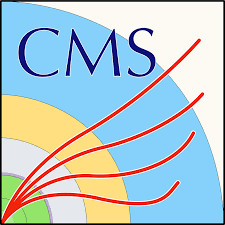
\includegraphics[width=1.0cm]{plots/CMS_Logo.png}
% % \includegraphics[width=1.0cm]{plots}
% }
\logo{
  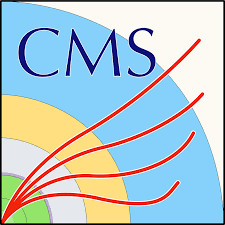
\includegraphics[width=0.7cm]{plots/CMS_Logo.png}
  
\includegraphics[width=0.7cm]{plots/CERN_logo.png}
}

%\author{Huiling Hua}
%\institute{IHEP}
% \institute[IHEP] % (optional)
% {
%   \inst{1}%
%     IHEP
% }
\date[14.04.2022] % (optional, should be abbreviation of conference name)
{HGC Si characterisations at CERN}

% - Either use conference name or its abbreviation.
% - Not really informative to the audience, more for people (including
%   yourself) who are reading the slides online
\subject{Physics Analysis}
% This is only inserted into the PDF information catalog. Can be left
% out. 

% If you have a file called "university-logo-filename.xxx", where xxx
% is a graphic format that can be processed by latex or pdflatex,
% resp., then you can add a logo as follows:
% \pgfdeclareimage[height=0.4.1cm]{university-logo}{university-logo-filename}
% \logo{\pgfuseimage{university-logo}}

% Delete this, if you do not want the table of contents to pop up at
% the beginning of each subsection:
% \AtBeginSubsection[]
% {
  % \begin{frame}<beamer>{Outline}
    % \tableofcontents[currentsection,currentsubsection]
  % \end{frame}
% }
\AtBeginSection[]
{
  \begin{frame}<beamer>{Outline}
    \tableofcontents[currentsection]
    % \addtocounter{framenumber}{-1}
  \end{frame}
}

\begin{document}

\begin{frame}
  \titlepage
\end{frame}

% \begin{frame}{Outline}
%   \tableofcontents
  % You might wish to add the option [pausesections]
% \end{frame}
\section{Introduction}


\begin{frame}{RINSC irradiation, overview}
  \begin{table}[htbp] %[h]
      \centering
      \footnotesize%Use \footnotesize for a 20% (linear) reduction in font size
      \setlength\tabcolsep{2pt}%Reduce the amount of intercolumn whitespace
      \resizebox{0.8\textwidth}{!}{% 
          \begin{tabular}{|c | c |c|} 
           \hline
              & \href{https://indico.cern.ch/event/1121372/contributions/4715417/attachments/2382784/4071626/2-1-2022_Irradiation_Update_from_Brown.pdf}{Round 5}   & \href{https://indico.cern.ch/event/1121372/contributions/4715417/attachments/2382784/4071626/2-1-2022_Irradiation_Update_from_Brown.pdf}{Round 6}\\

           \hline
           \textbf{Date}   & 19.01.2022 &  26.01.2022 \\
           \hline
           \textbf{Target fluence [neq/cm2]}  &   4.00E+15 & 5.50E+15\\
           \hline
           \href{https://indico.cern.ch/event/1121372/contributions/4715417/attachments/2382784/4071626/2-1-2022_Irradiation_Update_from_Brown.pdf}{\textbf{Annealing time in the reactor at $60^{oC}$}}  &  16.1 min & 115.4 min \\
           \hline
           \textbf{Order} (back to front) &   N4792\_08, N4790\_09, N4790\_21 & N4792\_09, N4790\_08, N4790\_20 \\
           \hline
          \end{tabular}
      }
      \end{table}
      
    \begin{columns}
        \column{.5\textwidth}
        \begin{figure}
          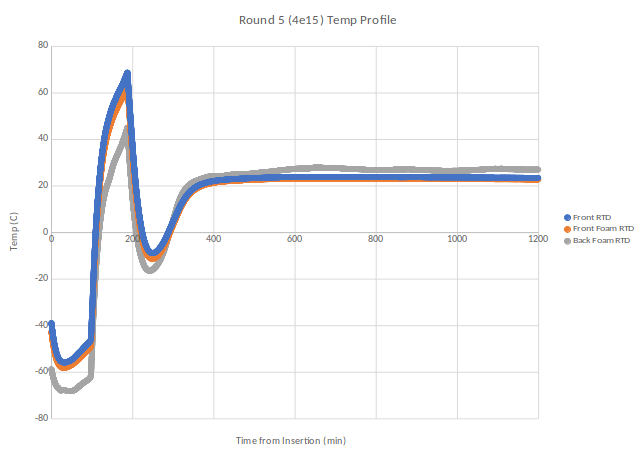
\includegraphics[width=0.9\textwidth]{plots/Round5_temp_profile.png}
          % \caption{Round 5, temperature profile}
        \end{figure}
        \column{.5\textwidth}
        \begin{figure}
          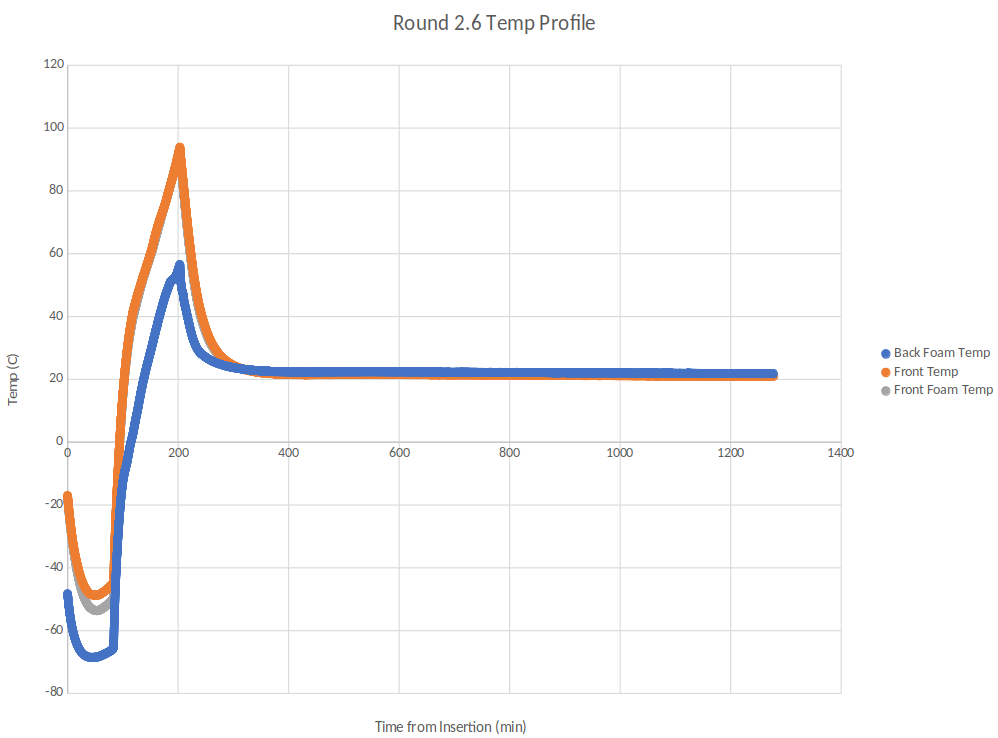
\includegraphics[width=.9\textwidth]{plots/Round6_temp_profile.png}
        \end{figure}
    \end{columns}
\end{frame}



\begin{frame}{Sensor list and annealing step}
%   \begin{figure}
%       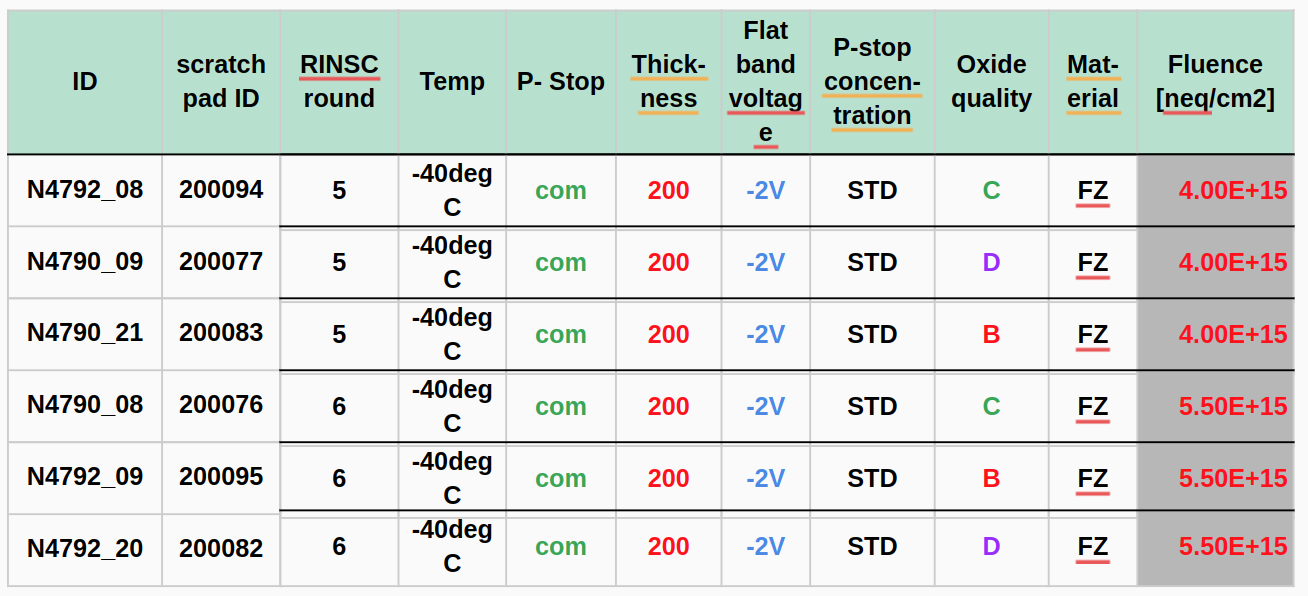
\includegraphics[width=.45\textwidth]{plots/Sensors.png}
%   \end{figure}

    \begin{table}[htbp] %[h]
        \centering
        \footnotesize%Use \footnotesize for a 20% (linear) reduction in font size
        \setlength\tabcolsep{2pt}%Reduce the amount of intercolumn whitespace
        \resizebox{1.0\textwidth}{!}{% 
            \begin{tabular}{|c | c |c|c|} 
             \hline
                sensor &  annealing steps post raditation & IV grading & CV grading \\
             \hline
             N4790\_09  & 27.6min + 31.8min & all passed & inclusive \\ 
             \hline
             N4790\_21 & 10.9min + 11.7min + 11.4min + 9.6min +11.5min + 19.9min+ 11.4min + 17.2min & all passed & inclusive  \\

             \hline
             N4792\_7 & 30.9min +  31.0min  & 0 passed , 30 analysis not run, 60 passed& inclusive \\
             \hline
             \hline
             N4790\_08 & no additional annealing & passed & inclusive \\
             N4792\_09 & no additional annealing & passed & inclusive \\
             N4792\_20 & no additional annealing & analysis not run & inclusive\\
            \hline
            \end{tabular}
        }
        \caption{Annealing steps}
        \end{table}   
  \begin{itemize}
      \small
      \item Sensor N4792\_08 could not be located, instead the sensor N4792\_07 was found in the stack
  \end{itemize}
\end{frame}


\begin{frame}{Measurement Setup: ALPS}
    \begin{figure}
        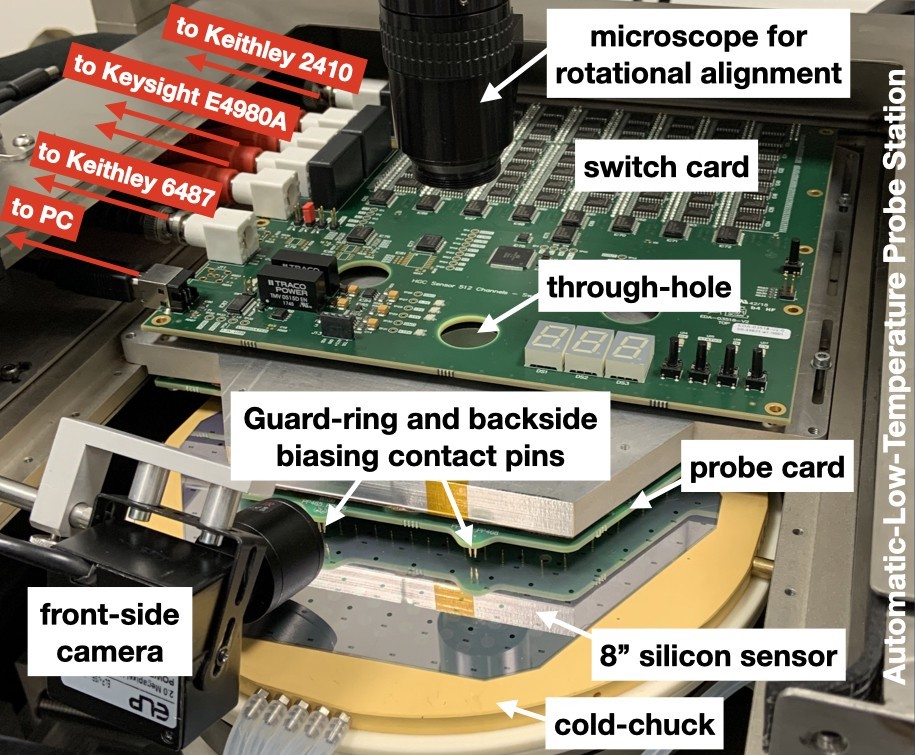
\includegraphics[width=.45\textwidth]{plots/ALPS_setup.png}
    \end{figure}
  
    \begin{itemize}
        % \small
        \scriptsize
        \item Sensors placed directly on chuck (no backside protection)
        \item Temperature: $-40^oC$; humidity: $ 4\% - 8\%$
        \item Voltage provided through the HV pin to the frontside;  voltage up to \alert{-850V}
        \item Annealing at $60^oC$ (chuck), target time of 115 mins
        \item Sensors from Round 5 were annealed to the total time of 115 min at CERN 
        \item Sensors from Round 6 were not further annealed
    \end{itemize}
\end{frame}
  

\section{IV Results, Annealing}


\begin{frame}{IV results, N4790\_21}
   \begin{columns}
        \column{.45\textwidth}
        \begin{figure}
            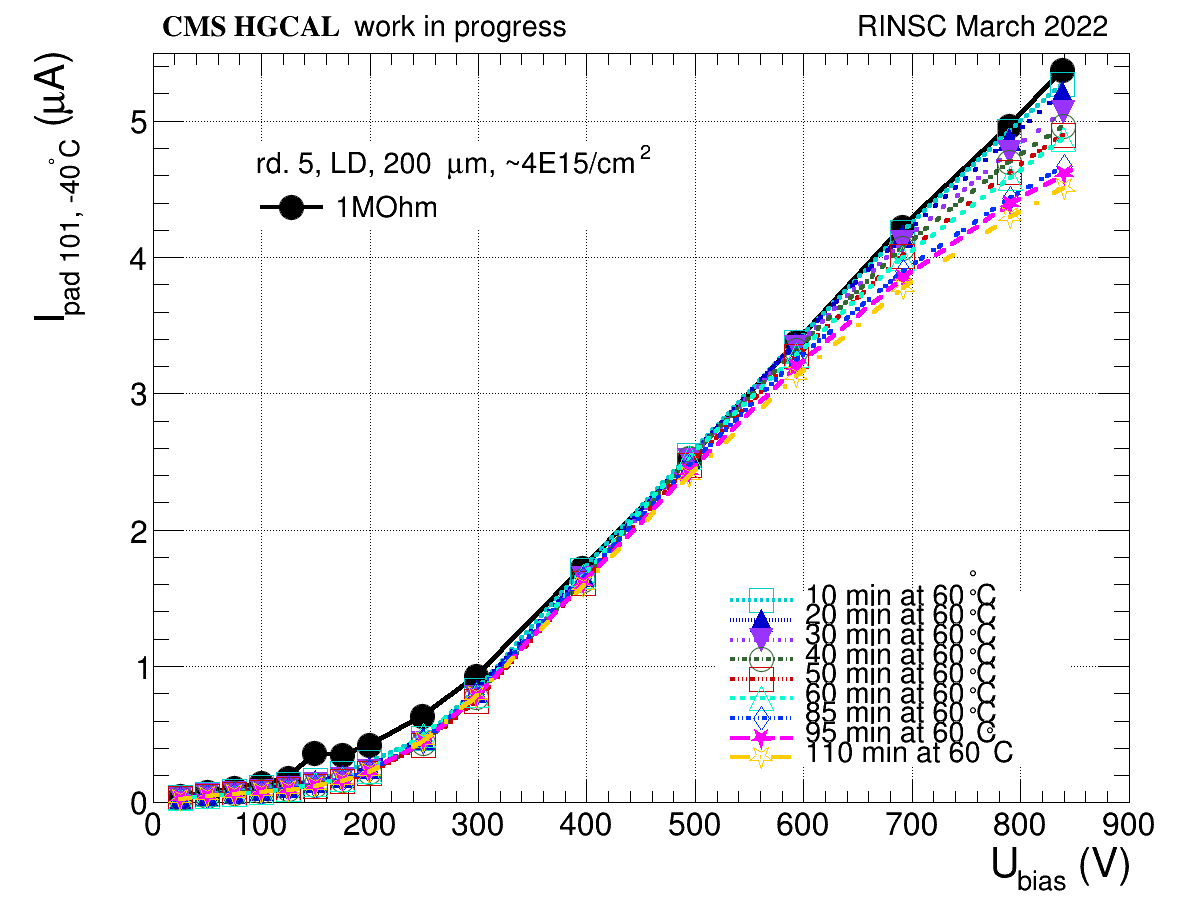
\includegraphics[width=1.0\textwidth]{plots/annealing_IV_ch101_N4790_21.png}
            \caption{IV of pad 101}
        \end{figure}

        \column{.55\textwidth}
        \begin{figure}
            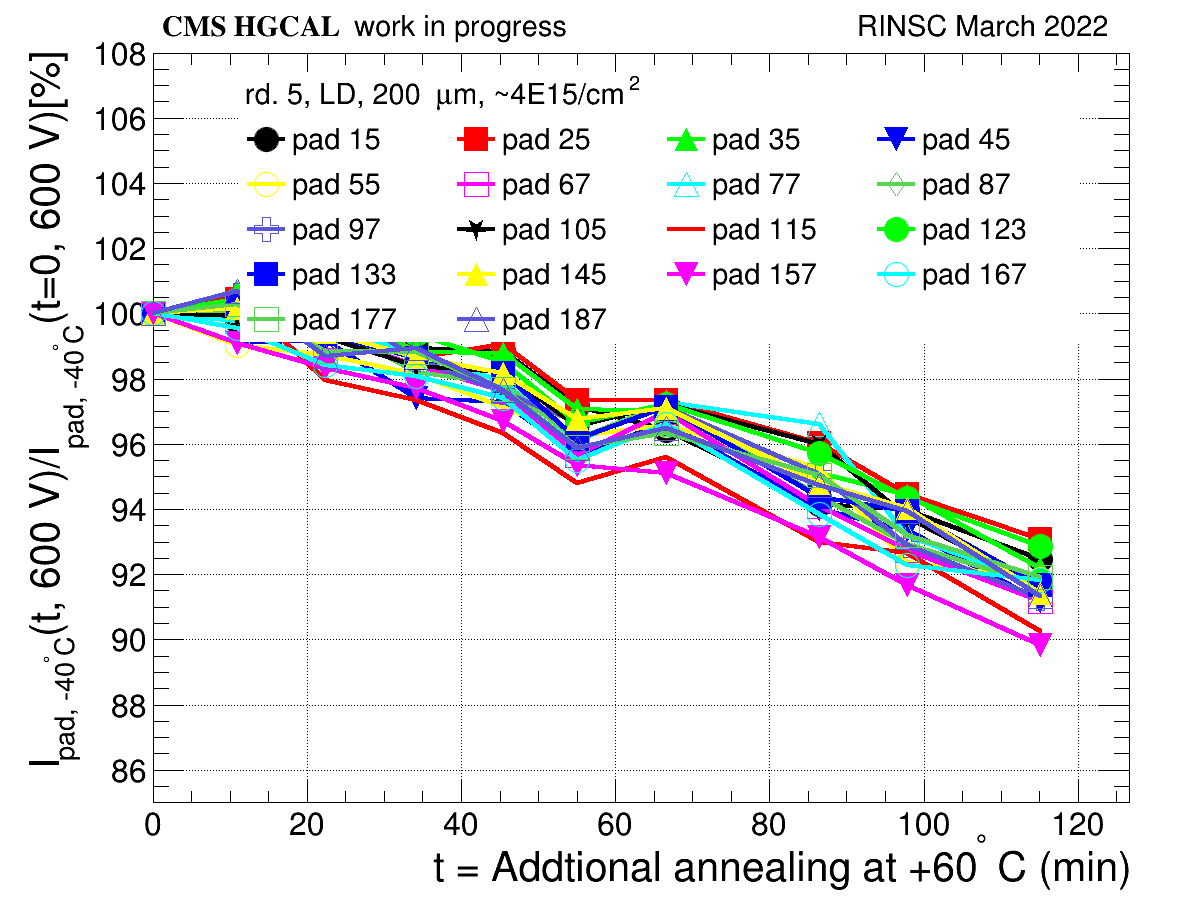
\includegraphics[width=1.0\textwidth]{plots/annealing_current_N4790_21.png}
            \caption{Current vs annealing time at 600V}
        \end{figure}
    \end{columns}
    \begin{itemize}
        \item we do see annealing effect on current
        \item plots of other channels in backup
    \end{itemize}
\end{frame}


\begin{frame}{IV results, N4790\_09 channel 101}
  \begin{columns}
       \column{.45\textwidth}
       \begin{figure}
           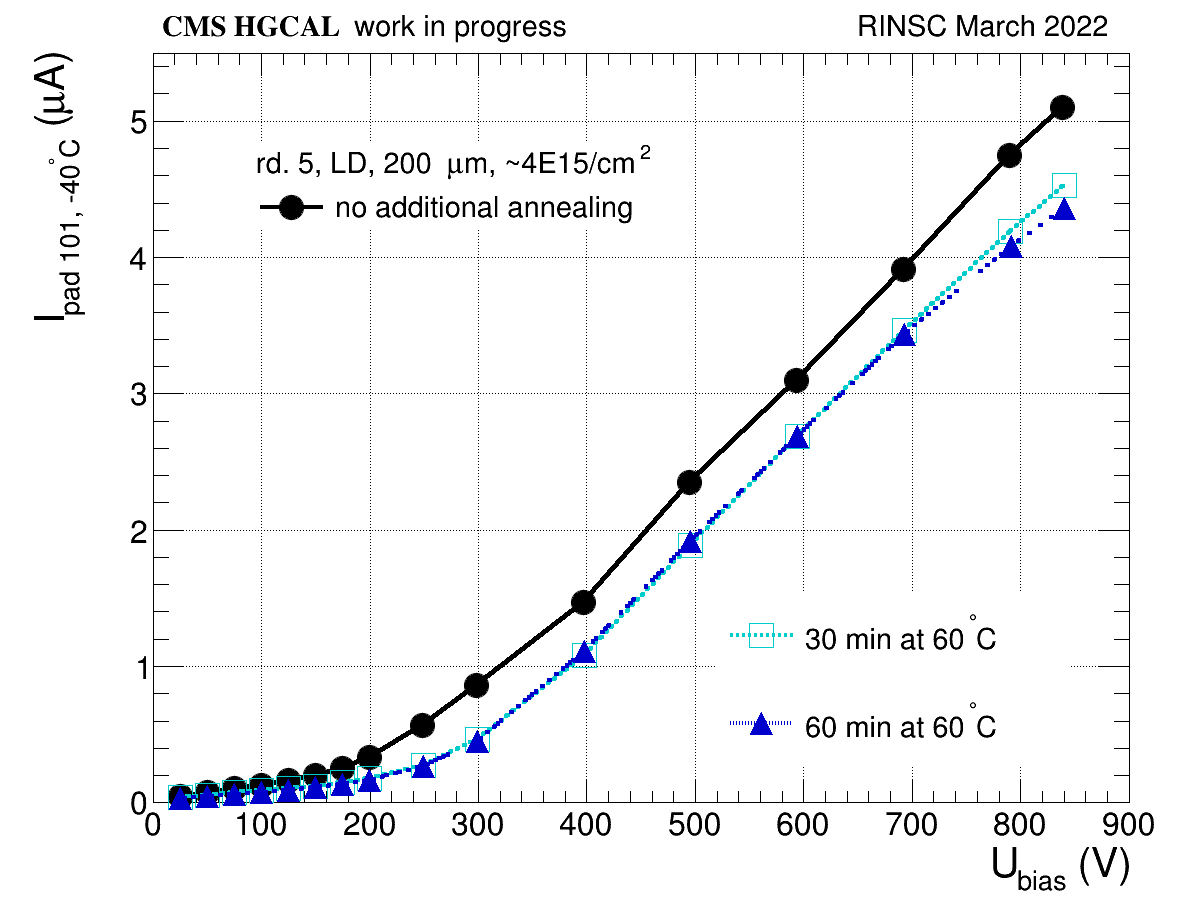
\includegraphics[width=1.0\textwidth]{plots/annealing_IV_ch101_N4790_09.png}
           \caption{Total current of all 19 HD sensors}
       \end{figure}
       \column{.55\textwidth}
       \begin{figure}
           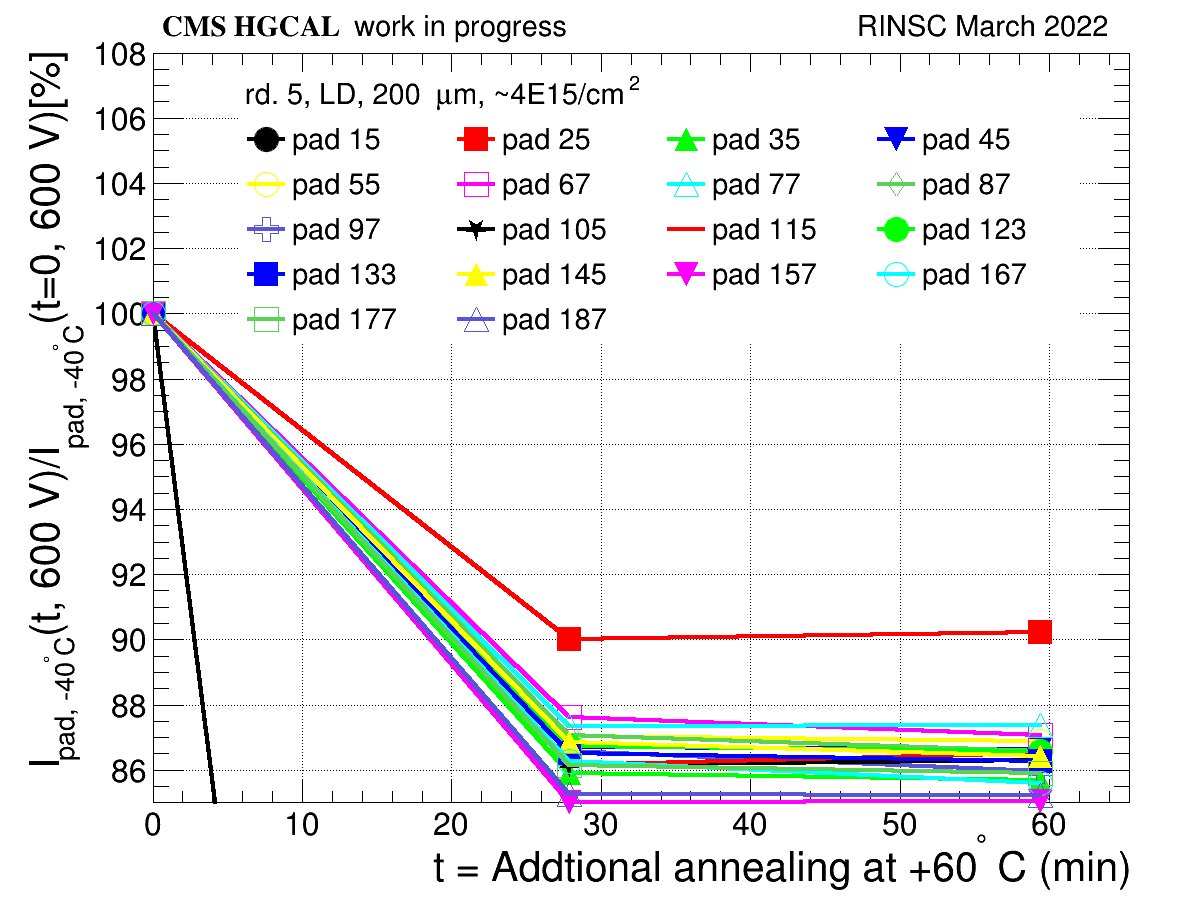
\includegraphics[width=1.0\textwidth]{plots/annealing_current_N4790_09.png}
           \caption{One of the failed sensors}
       \end{figure}
   \end{columns}
\end{frame}

\begin{frame}{IV results, N4792\_07}
  \begin{columns}
       \column{.45\textwidth}
       \begin{figure}
           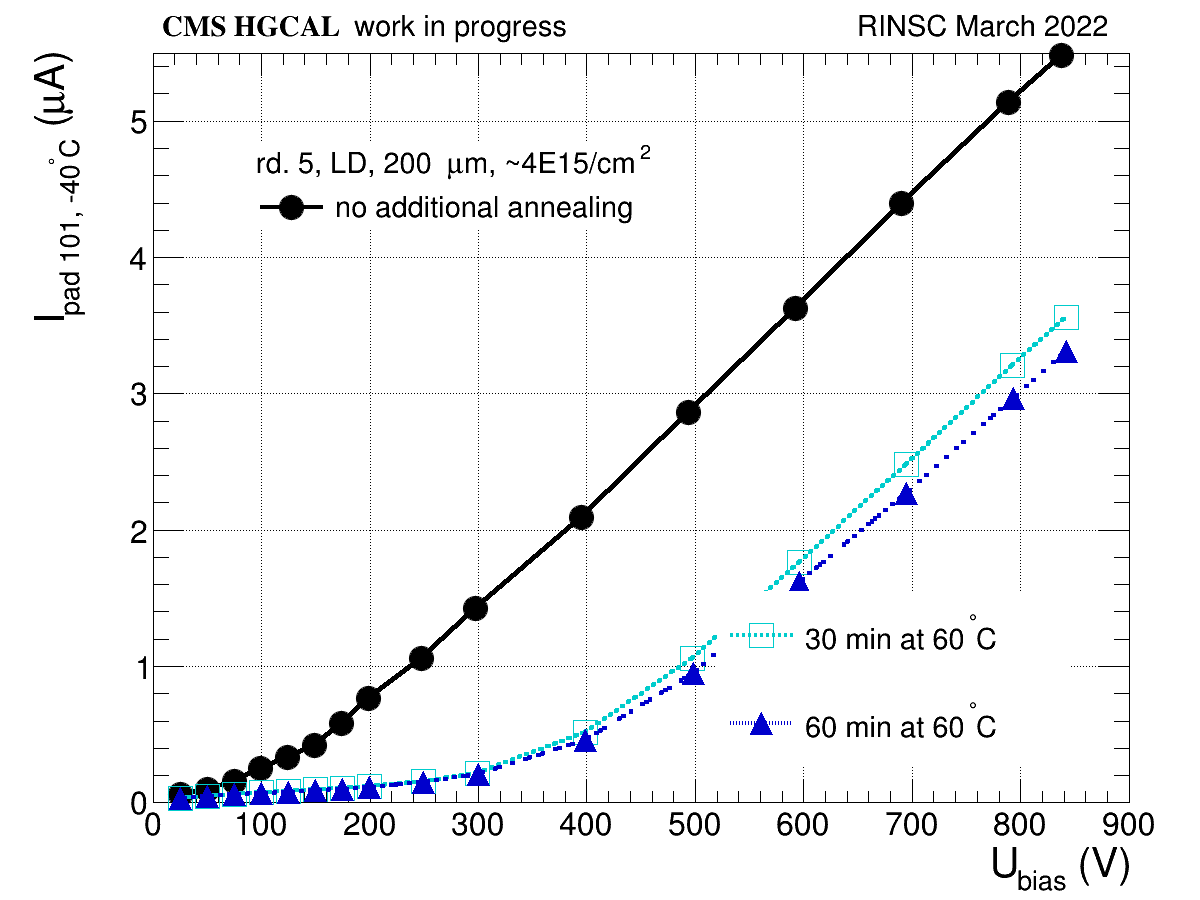
\includegraphics[width=1.0\textwidth]{plots/annealing_IV_ch101_N4792_7.png}
           \caption{Total current of all 19 HD sensors}
       \end{figure}

       \column{.55\textwidth}
       \begin{figure}
           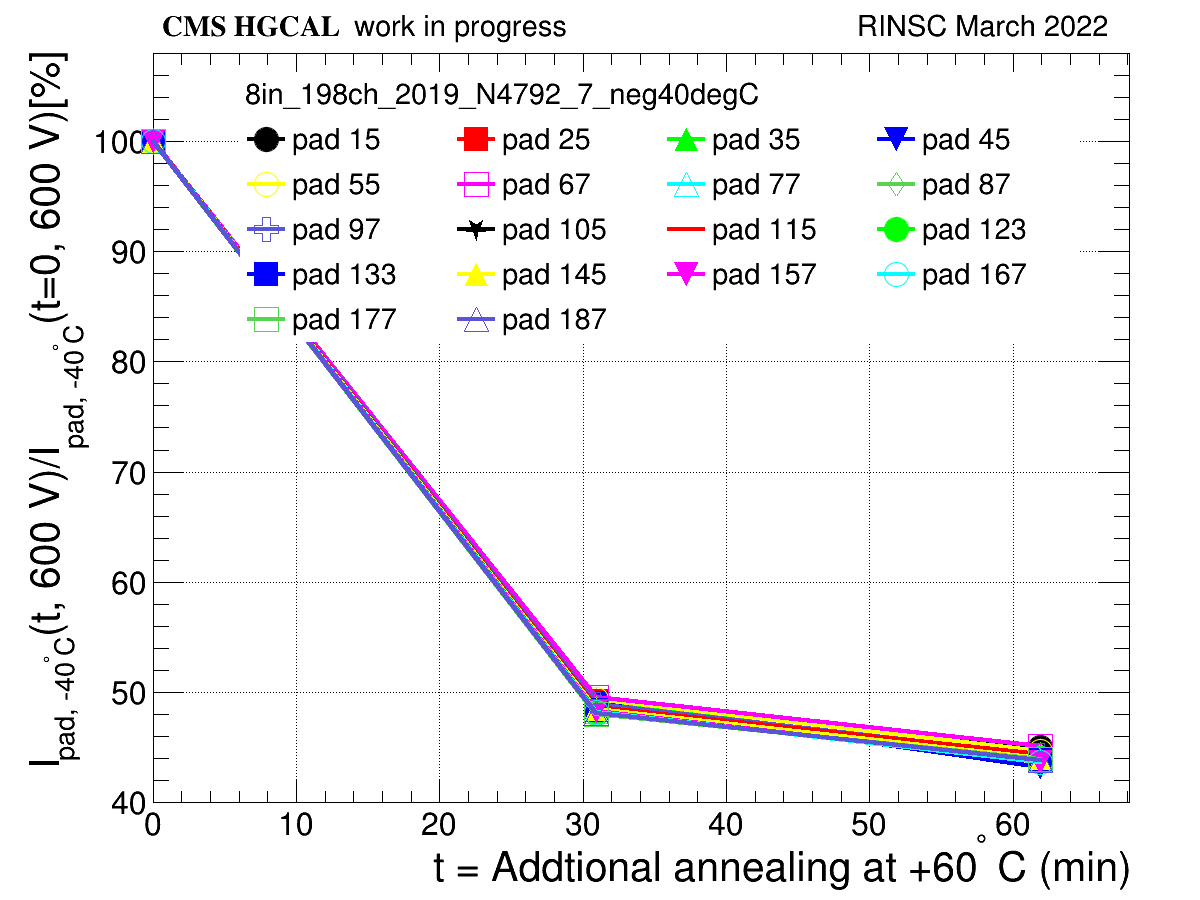
\includegraphics[width=1.0\textwidth]{plots/annealing_current_N4792_7.png}
           \caption{One of the failed sensors}
       \end{figure}
   \end{columns}
\end{frame}



\section{CV Results, Annealing}

\begin{frame}{CV results, N4790\_21}
  \begin{figure}
      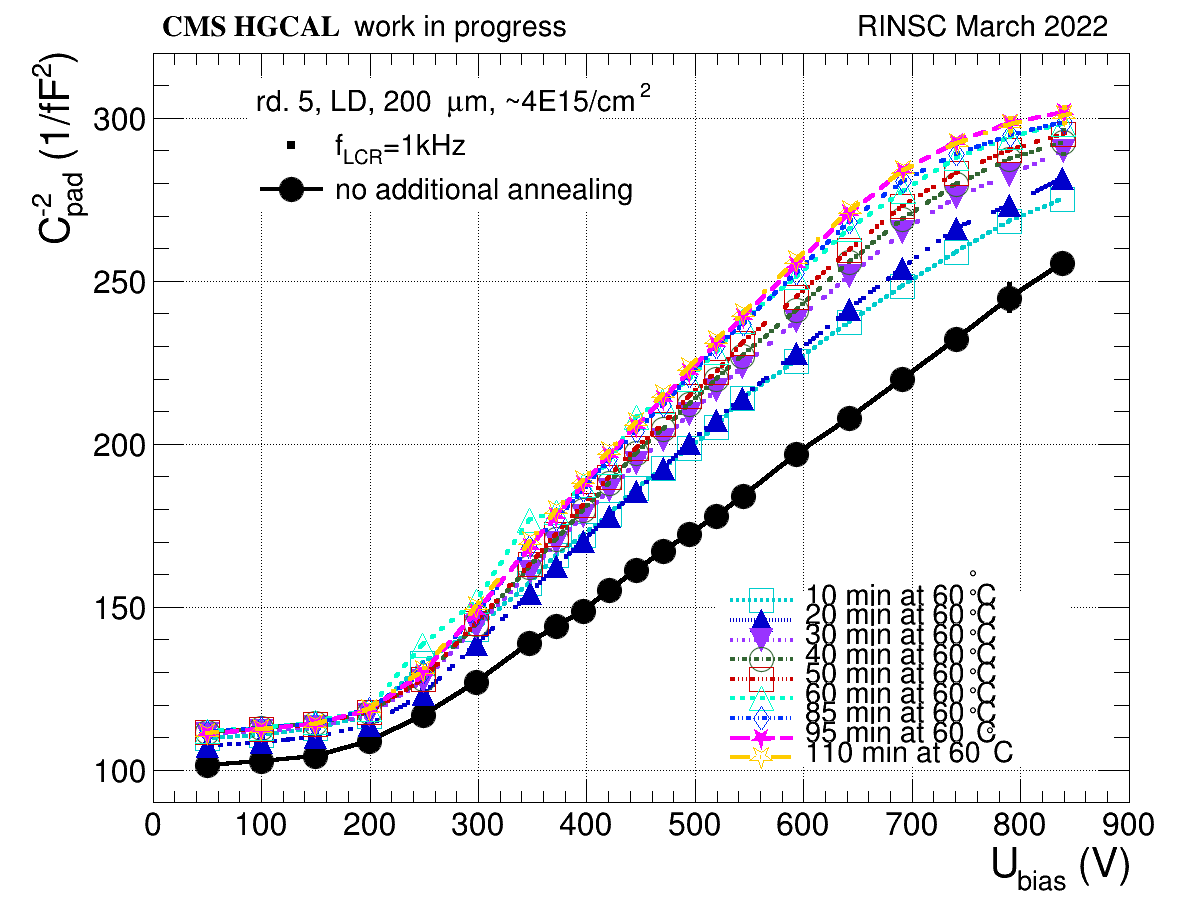
\includegraphics[width=.6\textwidth]{plots/annealing_CV_ch101_N4790_21.png}    
  \end{figure}
  \begin{itemize}
    % \item HexPlots as graphical representation of cell properties on the sensor
    \item We do see annealing effects
    \item Reached the limit of reversed annealing at around \alert{60 min}
    \item  Depletion voltage not reached 
  \end{itemize}
\end{frame}

\begin{frame}{CV results, N4790\_09}
  \begin{figure}
      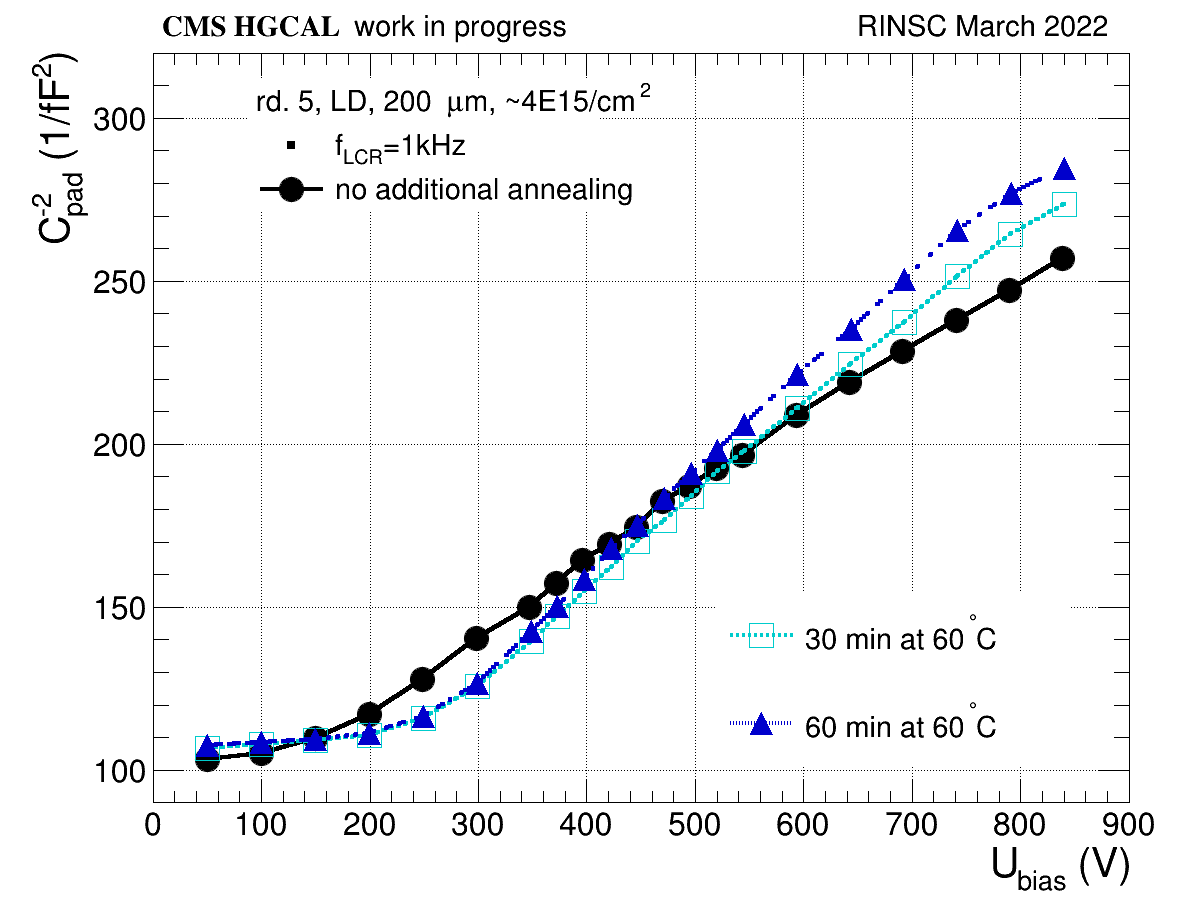
\includegraphics[width=.7\textwidth]{plots/annealing_CV_ch101_N4790_09.png}    
  \end{figure}
  \begin{itemize}
    \item CV curves
  \end{itemize}
\end{frame}

\begin{frame}{CV results, N4792\_07}
  \begin{figure}
      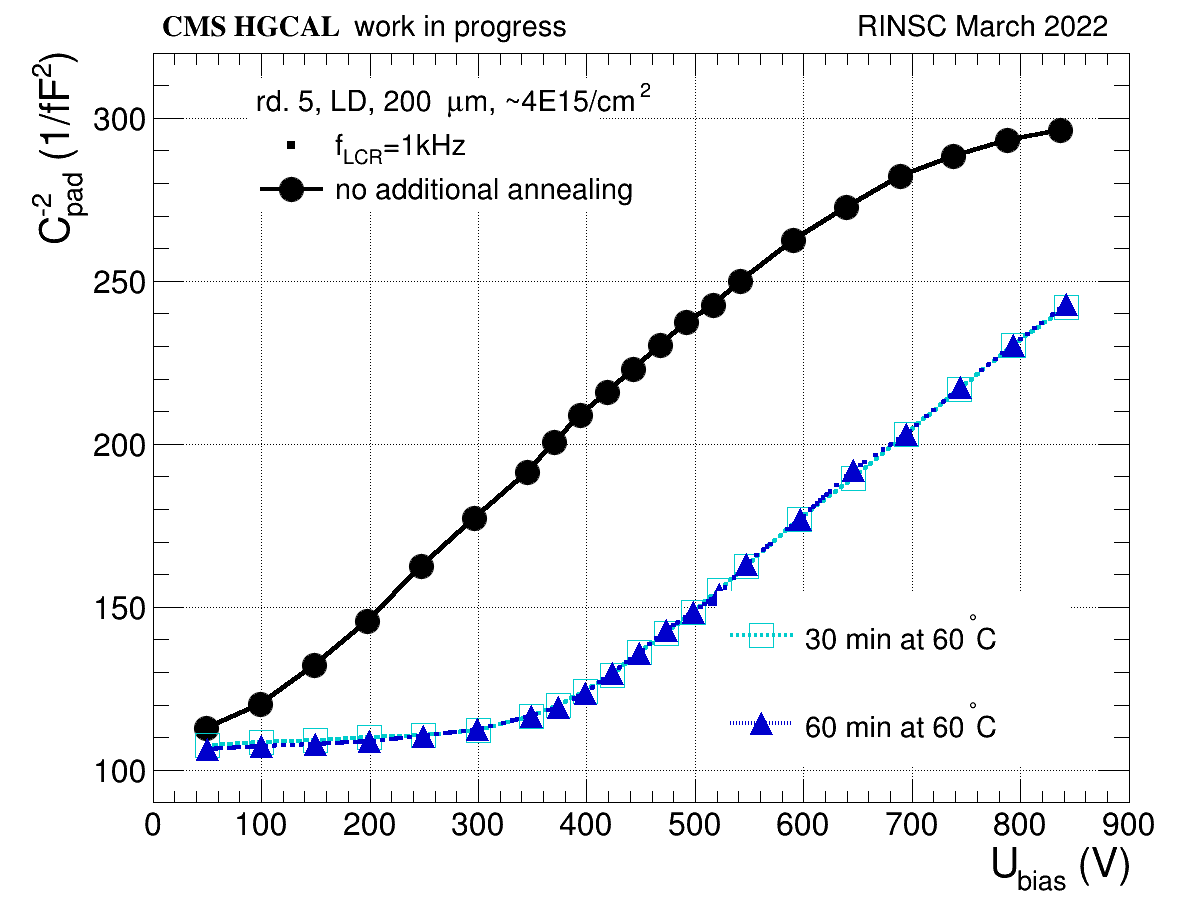
\includegraphics[width=.7\textwidth]{plots/annealing_CV_ch101_N4792_7.png}    
  \end{figure}
  \begin{itemize}
    \item CV curves
  \end{itemize}
\end{frame}



\section{Temperature effect}

\begin{frame}{Temperation effect on IV measurement}
    \begin{columns}
        \column{.5\textwidth}
        \begin{figure}
            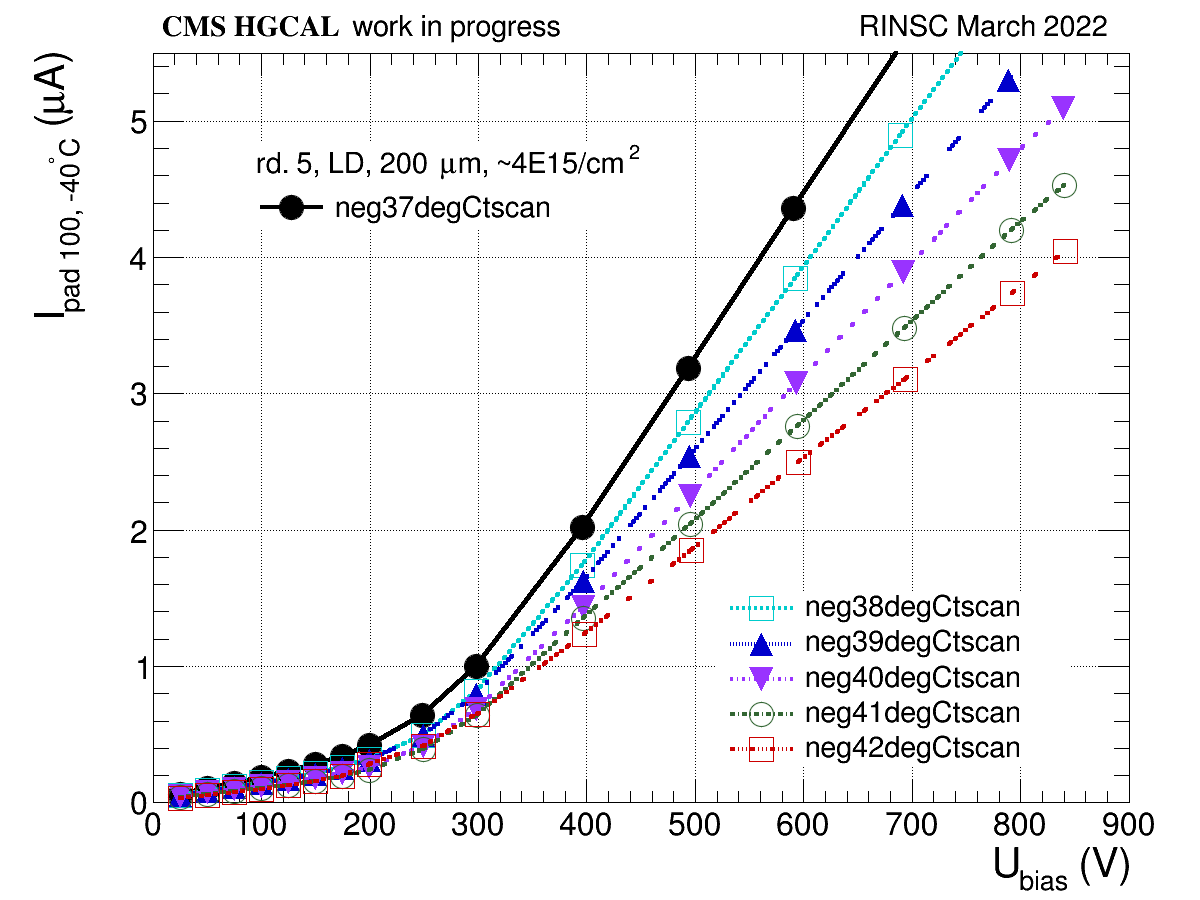
\includegraphics[width=1.0\textwidth]{plots/8in_198ch_2019_N4790_21_4E15_tempareture_effect_100.png}
        \end{figure}
        \column{.5\textwidth}
        \begin{figure}
            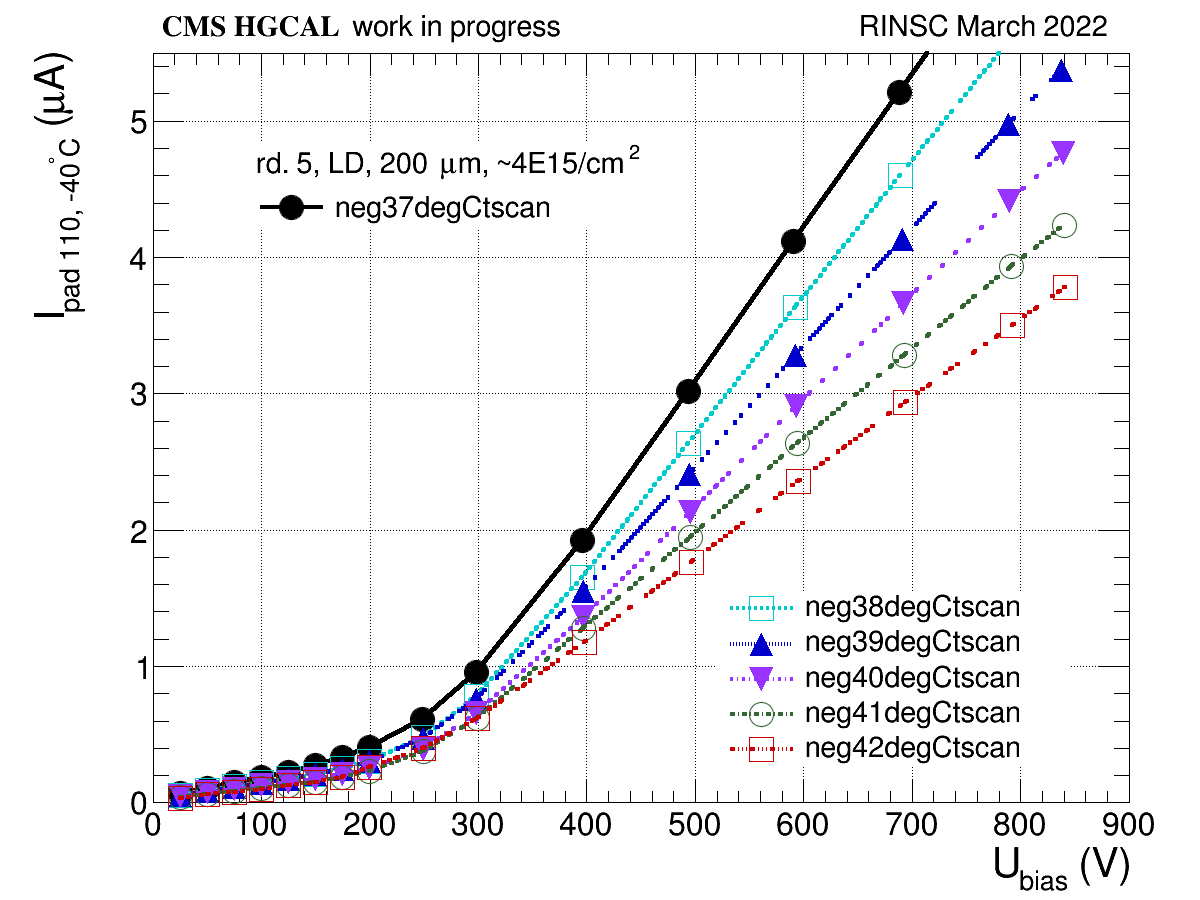
\includegraphics[width=1.0\textwidth]{plots/8in_198ch_2019_N4790_21_4E15_tempareture_effect_110.png}
        \end{figure}
    \end{columns}
\end{frame}

\begin{frame}{Temperature effect on CV measurement}
\end{frame}


\section{Alpha plot}

\begin{frame}{Proto-A: example CV results}
  \begin{figure}
      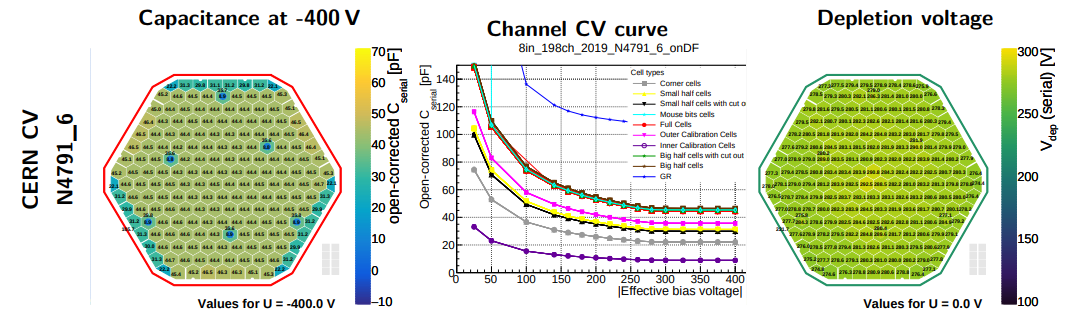
\includegraphics[width=1.0\textwidth]{plots/CV_example.png}    
  \end{figure}
  \begin{itemize}
    \item HexPlots as graphical representation of cell properties on the sensor
    \item CV curves
  \end{itemize}
\end{frame}

% \section{Additional Measurements}


% \begin{frame}{Longterm Leakage current stability}
%   \begin{figure}
%     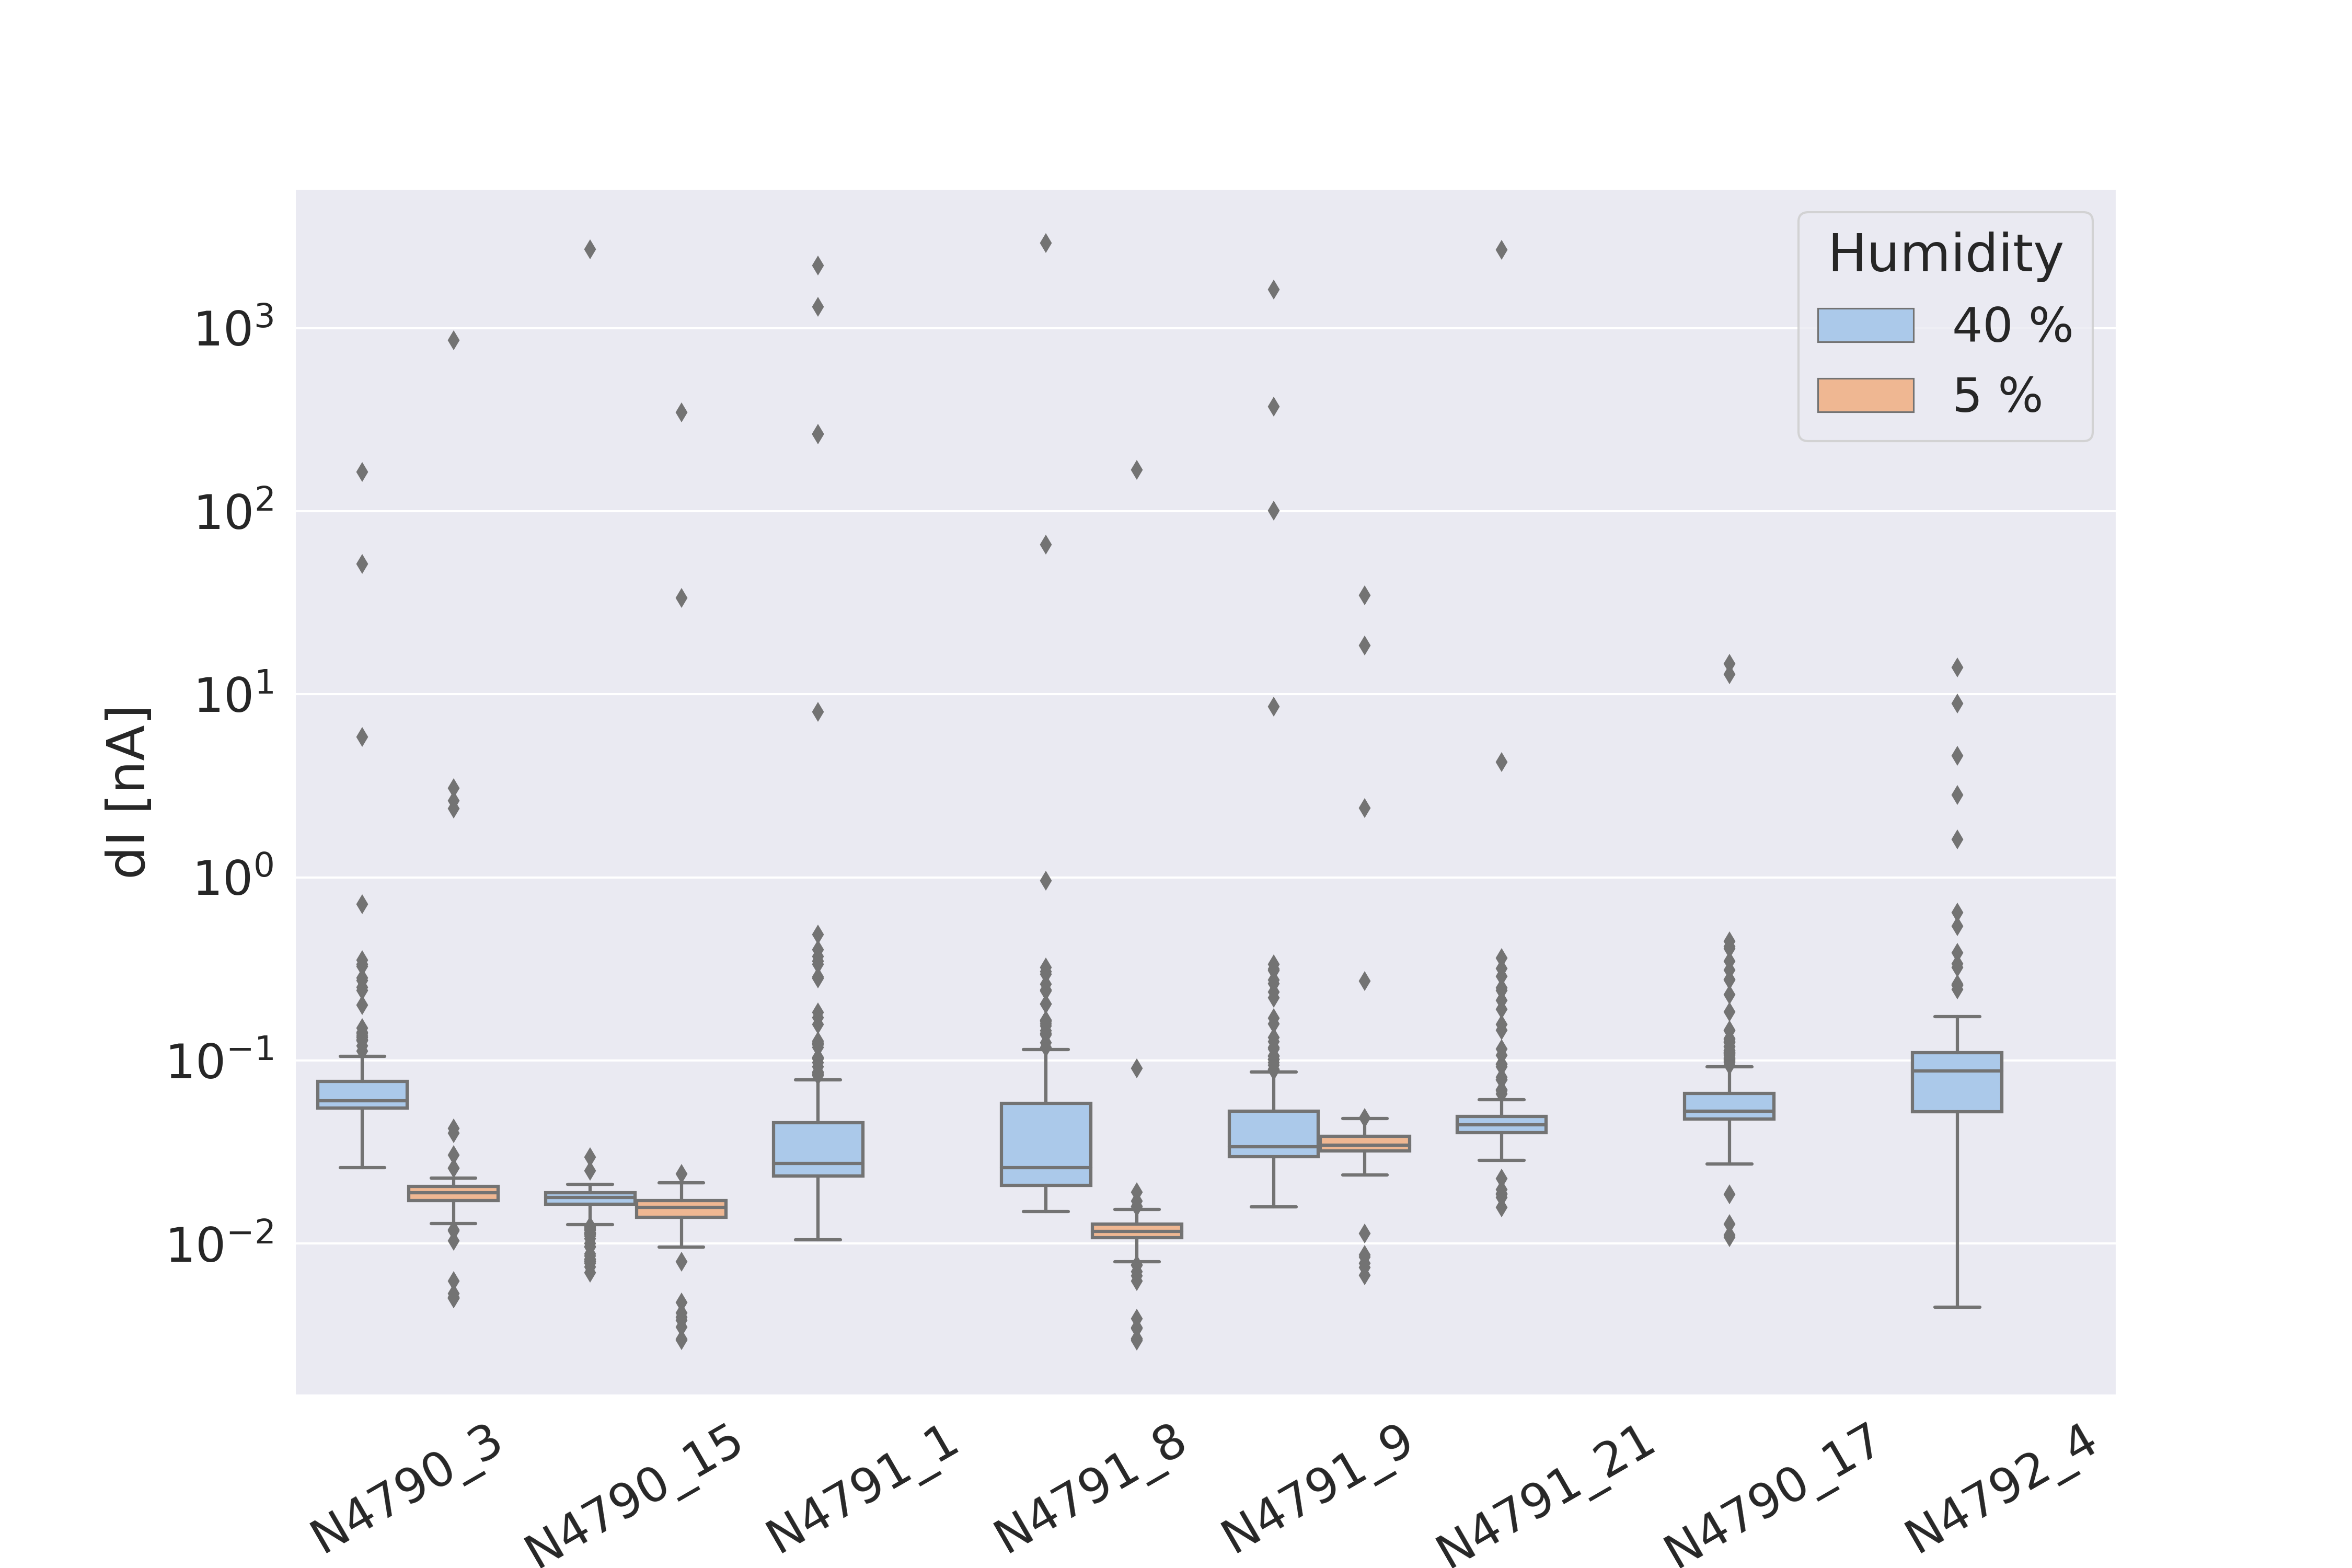
\includegraphics[width=.8\textwidth]{plots/RangesForCurrentVariationsDryAir.png}
%   \end{figure}
%   \href{https://indico.cern.ch/event/1121372/contributions/4708329/attachments/2382634/4071804/Longterm_Leakage_Current_Measurements.pdf}{\beamergotobutton{Longterm Current}}
% \end{frame}

% \begin{frame}{Dicing Frame removal at CERN}
%   \begin{columns}
%     \column{.5\textwidth}
%     \begin{figure}
%       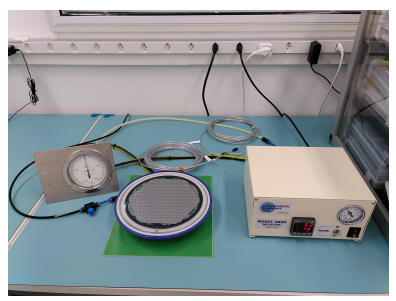
\includegraphics[width=1.0\textwidth]{plots/DF_removal_Picture.png}
%       \caption{Dicing Frame Removal Process at CERN}
%     \end{figure}

%     \column{.55\textwidth}
%     \begin{itemize}
%       \item Process Parameters:
%       \begin{itemize}
%         \item UV illumination
%         \item Temperature: $50  ^oC$
%         \item 600 mbar vacuum
%       \end{itemize}
%       \item Result:
%       \begin{itemize}
%         \item For the 300 um sensors 6 of previously 11 good sensors failed the IV requirements
%         \item 120 um and 200 um sensors were delivered off-DF
%       \end{itemize}
%     \end{itemize}

% \end{columns}

% \begin{figure}
% \end{figure} 
%   \href{https://indico.cern.ch/event/1085830/contributions/4565314/attachments/2344490/3998306/IVCV_recent_HGCal_prototype_sensors_Readiness_Review.pdf}{\beamergotobutton{Dicing Frame (Slide 24)}}
% \end{frame}

\section{Summary}
\begin{frame}{Summary}
  \begin{itemize}
    % \scriptsize
    \item Majority of sensors have good IV results
    \item CV results are good for all proto-A sensors
    \item Longterm leakage current instability can be observed  for some channels
    \item No discharges has been observed for proto A sensors
    % \item Test throughput 20 sensors per week
    % \item Shortage of LCR meters problem resolved
  \end{itemize}
\end{frame}

\appendix

\begin{frame}{Backup}
	\center
	\huge
	Backup slides
\end{frame}

\begin{frame}{IV results, N4790\_09 cat 650V and 700V}
  \begin{columns}
       \column{.45\textwidth}
       \begin{figure}
           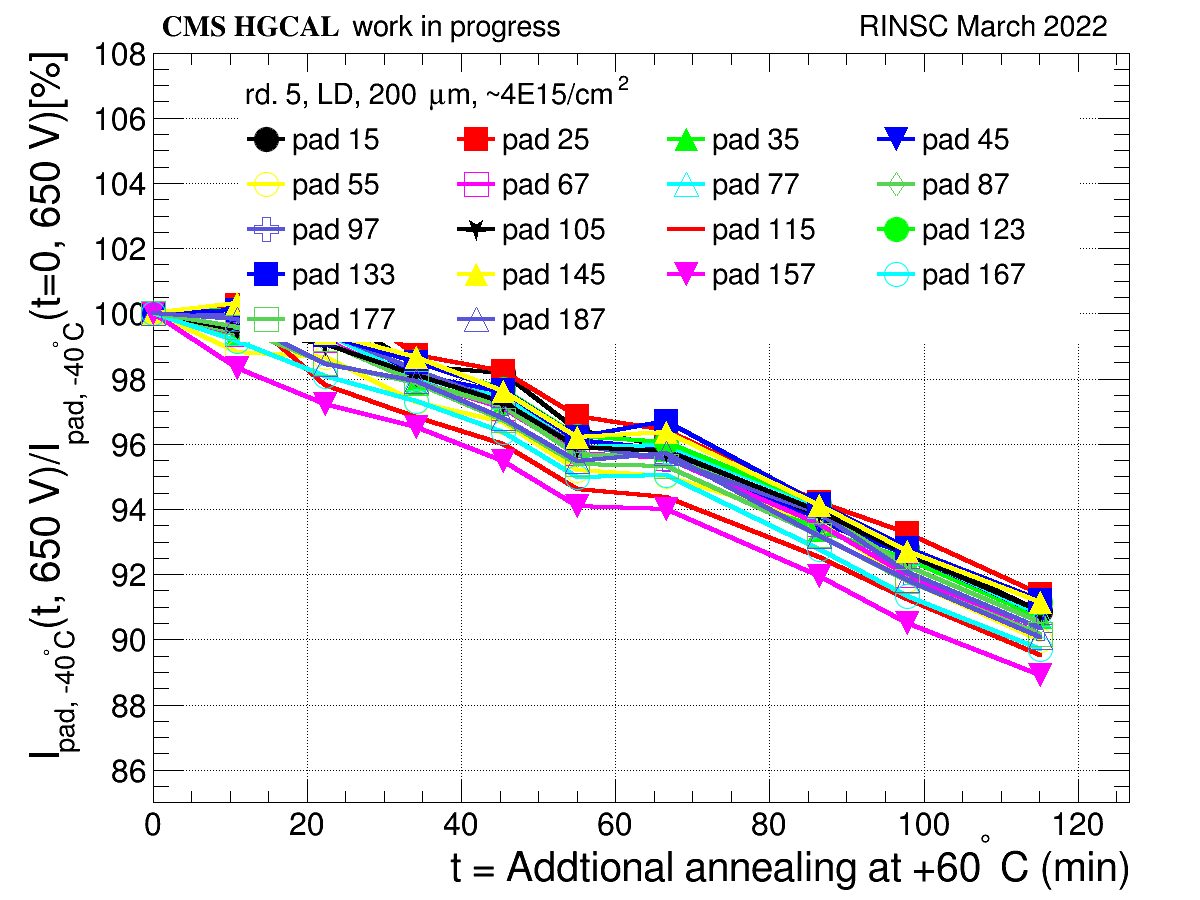
\includegraphics[width=1.0\textwidth]{plots/8in_198ch_2019_N4790_21_4E15_neg40degC_annealing_current_650.png}
       \end{figure}
       \column{.55\textwidth}
       \begin{figure}
           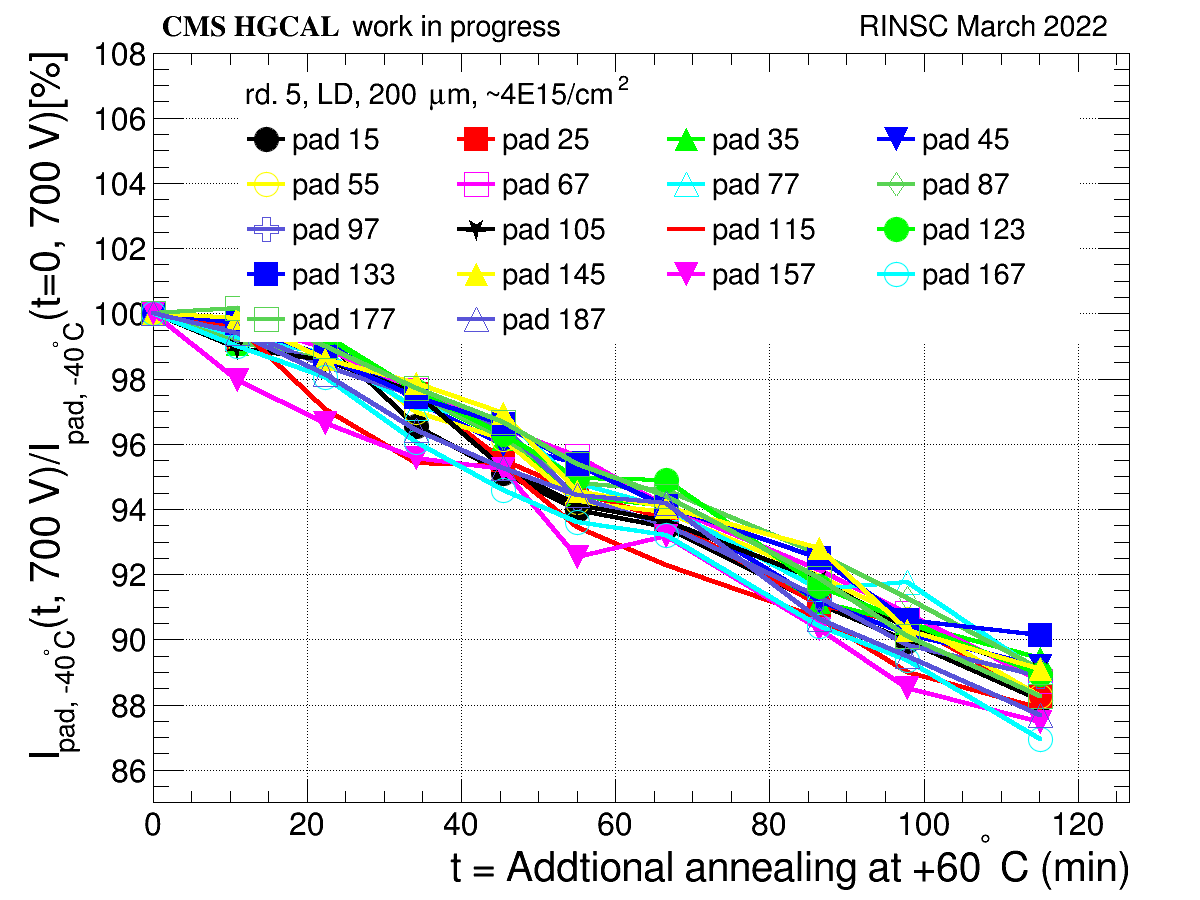
\includegraphics[width=1.0\textwidth]{plots/8in_198ch_2019_N4790_21_4E15_neg40degC_annealing_current_700.png}
       \end{figure}
   \end{columns}
\end{frame}

\begin{frame}{IV results, N4790\_09  650V and 700V}
  \begin{columns}
       \column{.45\textwidth}
       \begin{figure}
           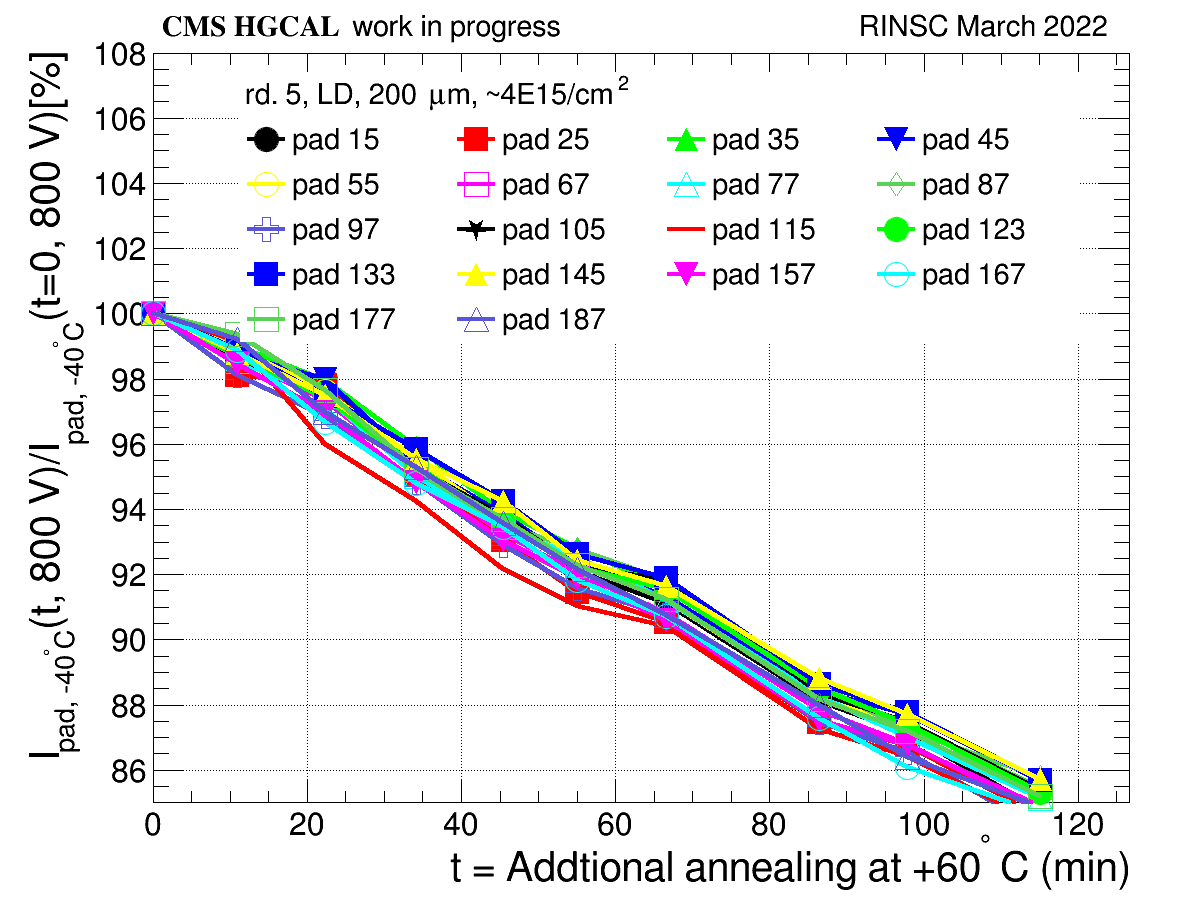
\includegraphics[width=1.0\textwidth]{plots/8in_198ch_2019_N4790_21_4E15_neg40degC_annealing_current_800.png}
       \end{figure}
       \column{.55\textwidth}
    %    \begin{figure}
        %    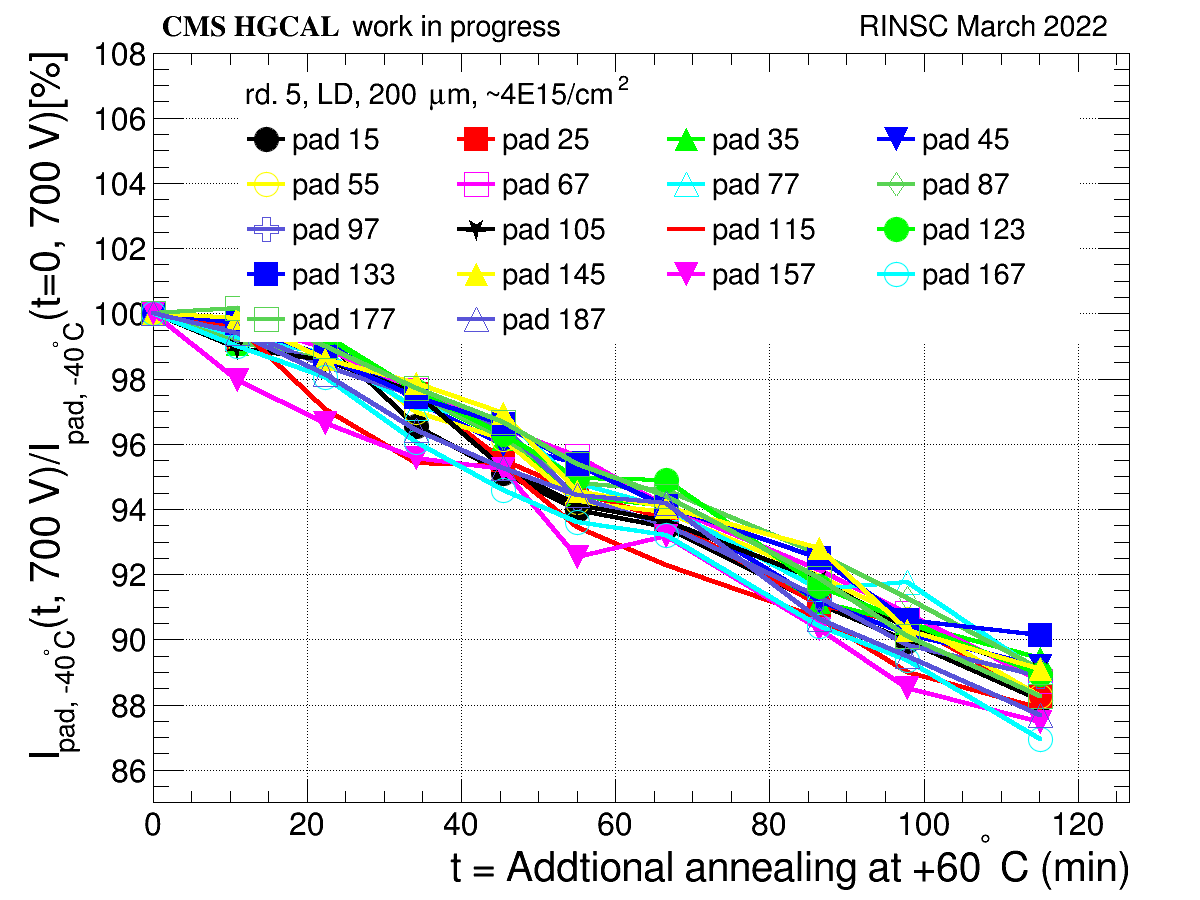
\includegraphics[width=1.0\textwidth]{plots/8in_198ch_2019_N4790_21_4E15_neg40degC_annealing_current_700.png}
    %    \end{figure}
   \end{columns}
\end{frame}

\begin{frame}{IV results, N4790\_09 }
  \begin{columns}
       \column{.45\textwidth}
       \begin{figure}
           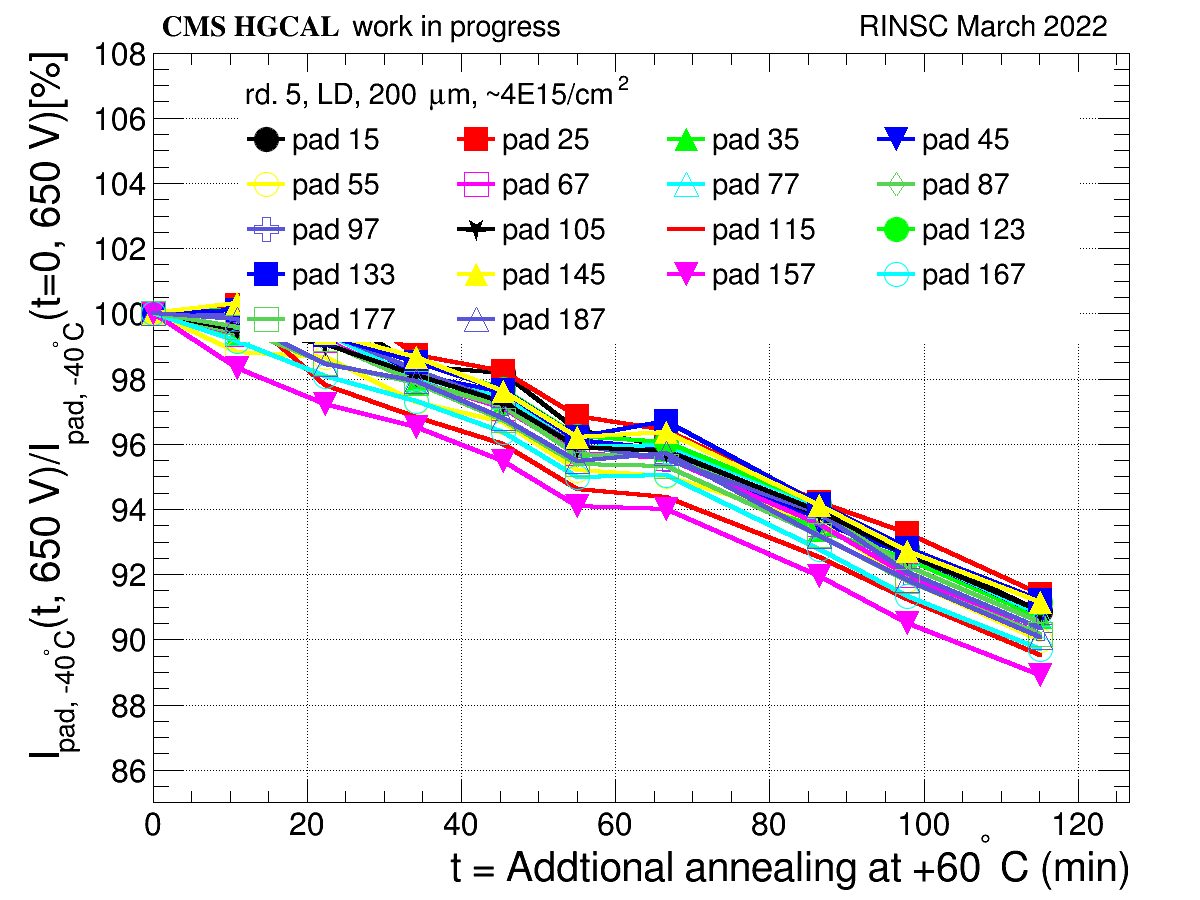
\includegraphics[width=1.0\textwidth]{plots/8in_198ch_2019_N4790_21_4E15_neg40degC_annealing_current_650.png}
       \end{figure}
       \column{.55\textwidth}
       \begin{figure}
           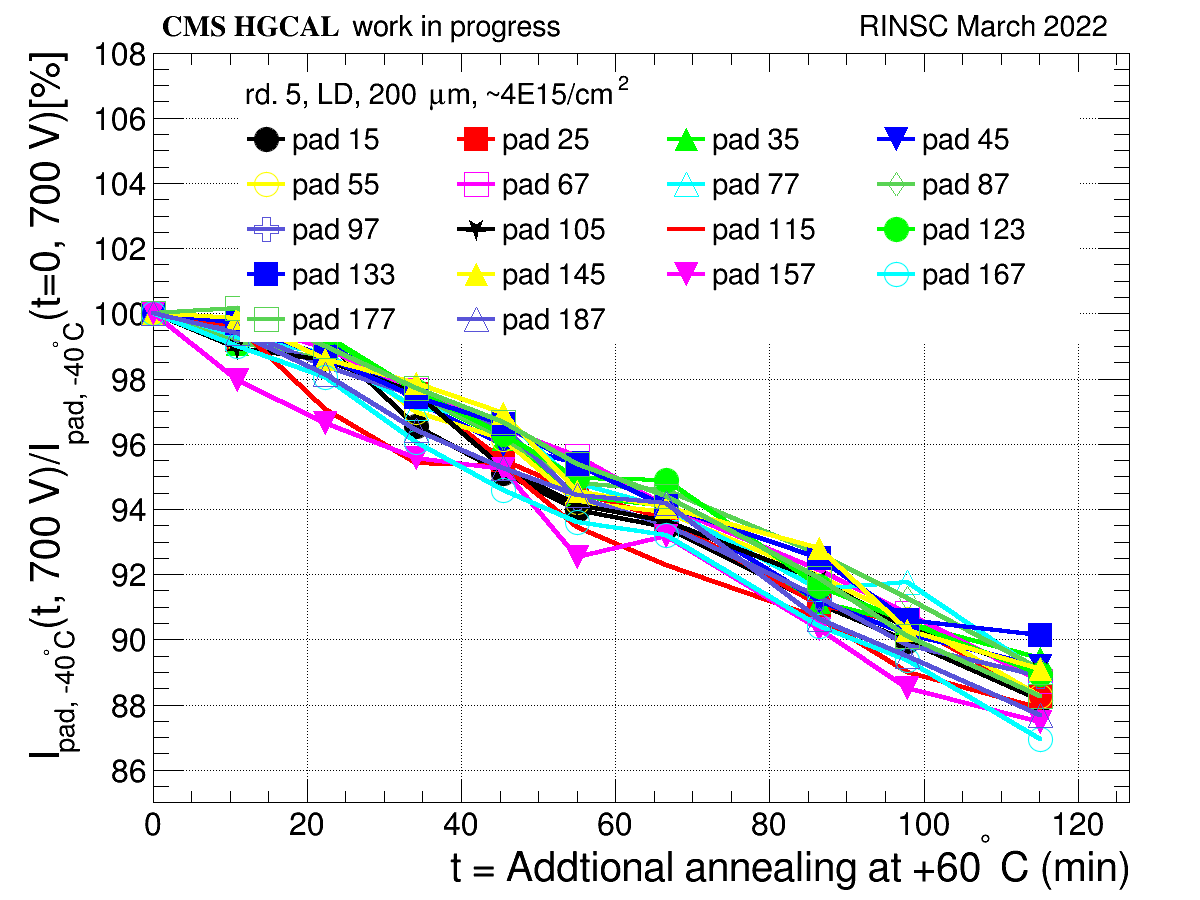
\includegraphics[width=1.0\textwidth]{plots/8in_198ch_2019_N4790_21_4E15_neg40degC_annealing_current_700.png}
       \end{figure}
   \end{columns}
\end{frame}

\begin{frame}{IV results, N4790\_09 channel at 650V and 700V}
  \begin{columns}
       \column{.45\textwidth}
       \begin{figure}
           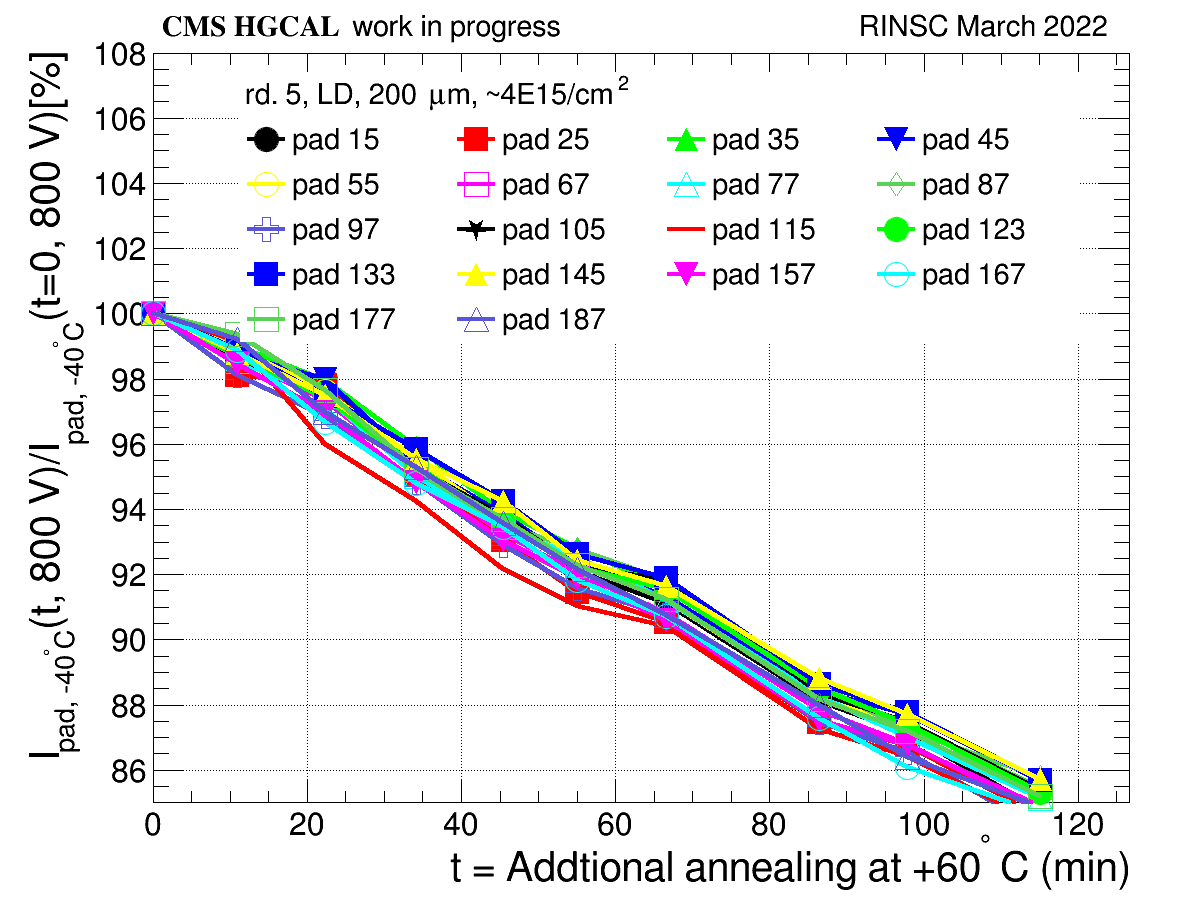
\includegraphics[width=1.0\textwidth]{plots/8in_198ch_2019_N4790_21_4E15_neg40degC_annealing_current_800.png}
       \end{figure}
       \column{.55\textwidth}
    %    \begin{figure}
        %    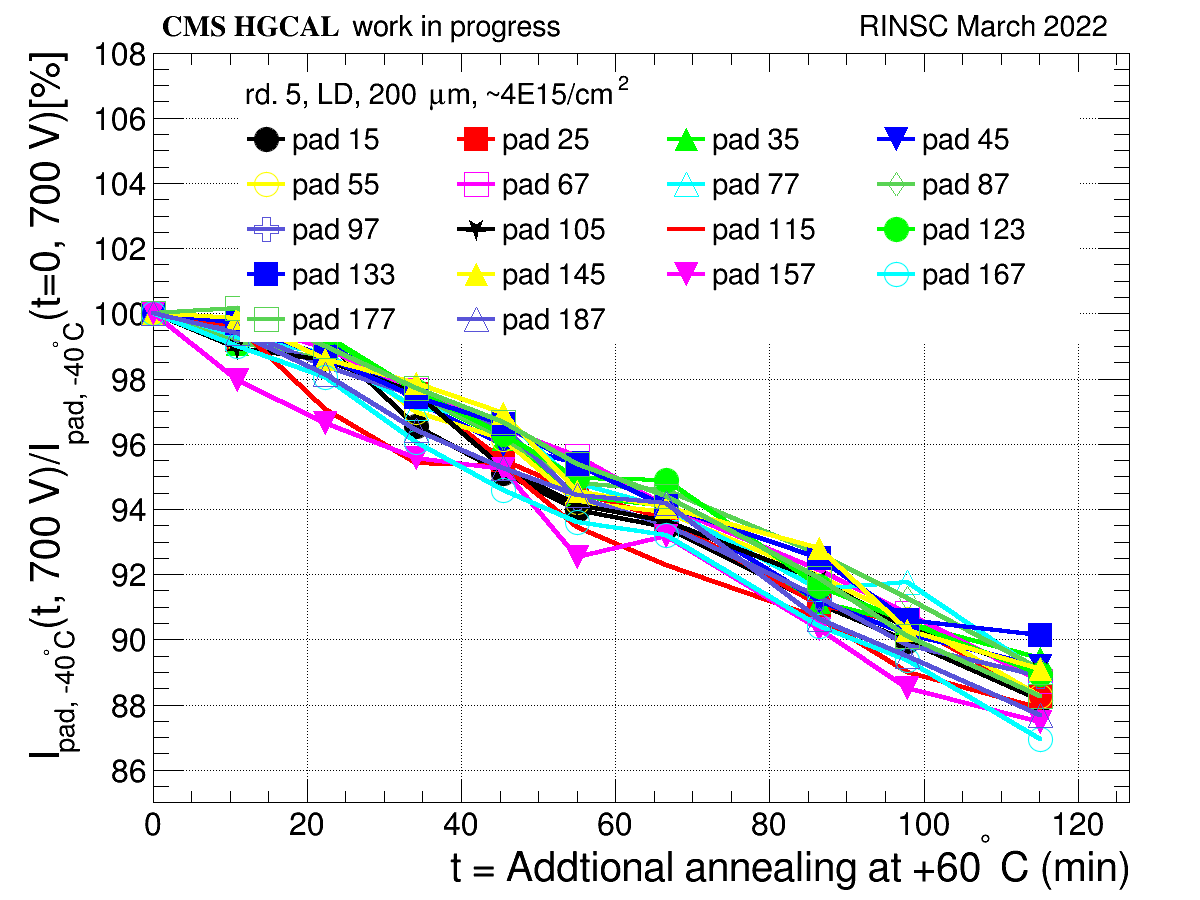
\includegraphics[width=1.0\textwidth]{plots/8in_198ch_2019_N4790_21_4E15_neg40degC_annealing_current_700.png}
    %    \end{figure}
   \end{columns}
\end{frame}



\begin{frame}{RINSC irradiation, Round 5}
  % \begin{itemize}
  %     \item Have measured \alert{43 sensors}
  %     \item 19 high density(HD) sensors(120um) 
  %     \item 26 low density(LD) sensors(12 with 200um and 14 with 300 um)
  % \end{itemize}

    \begin{figure}
        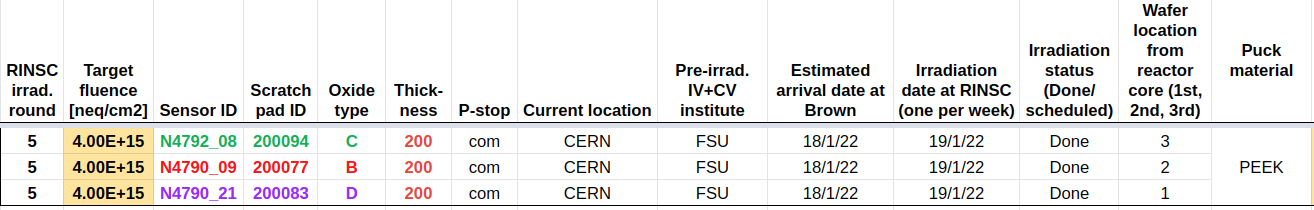
\includegraphics[width=.7\textwidth]{plots/Round_5_sensors.png}
        \caption{Round 5, sensors, N4792\_7 instead of N4792\_8}
    \end{figure}
    \begin{figure}
      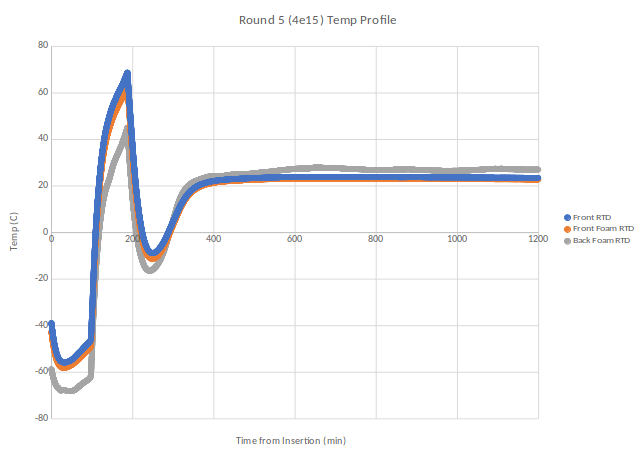
\includegraphics[width=.5\textwidth]{plots/Round5_temp_profile.png}
      \caption{Round 5, temperature profile}
    \end{figure}
\end{frame}

\begin{frame}{RINSC irradiation, Round 6}
  % \begin{itemize}
  %     \item Have measured \alert{43 sensors}
  %     \item 19 high density(HD) sensors(120um) 
  %     \item 26 low density(LD) sensors(12 with 200um and 14 with 300 um)
  % \end{itemize}

    \begin{figure}
        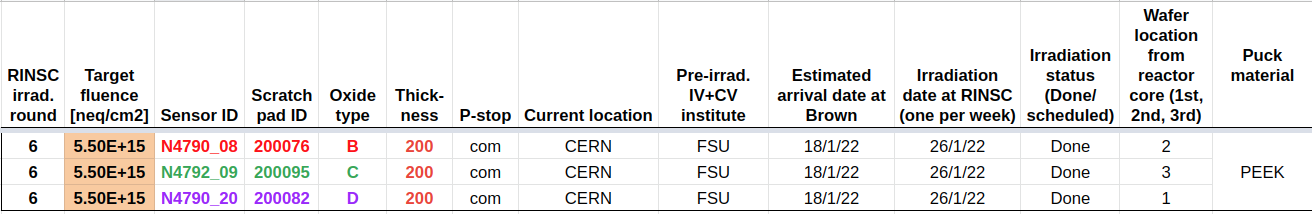
\includegraphics[width=.7\textwidth]{plots/Round_6_sensors.png}
        \caption{Round 6, sensors}
    \end{figure}
    \begin{figure}
      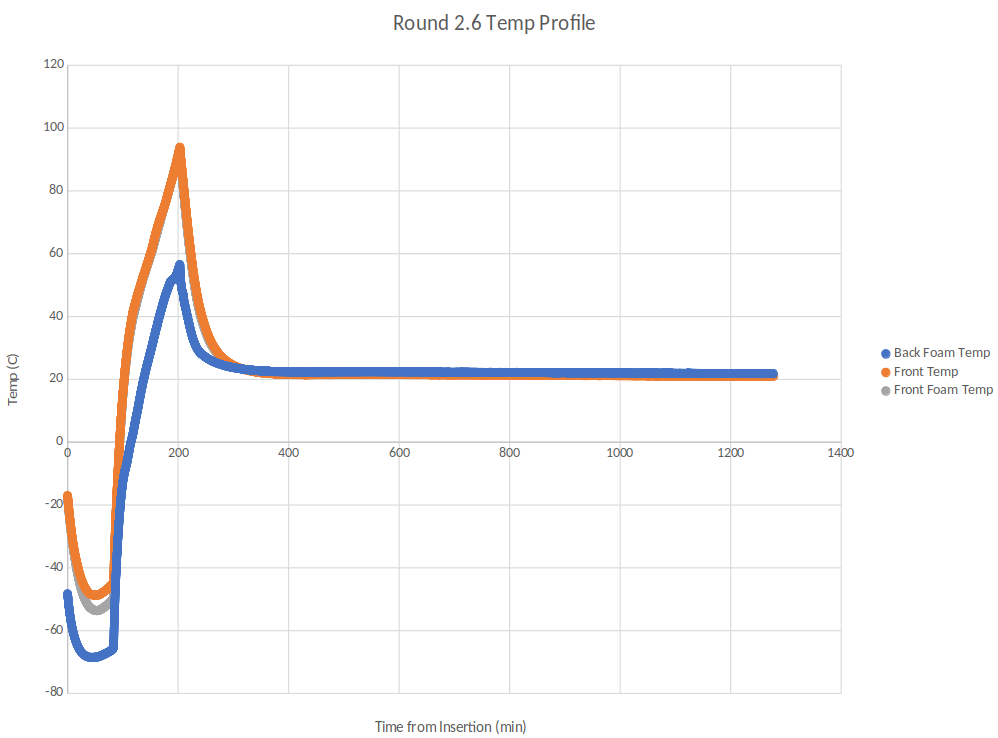
\includegraphics[width=.5\textwidth]{plots/Round6_temp_profile.png}
      \caption{Round 6, temperature profile}
    \end{figure}
\end{frame}

% \begin{frame}{Sensor list: HD}
%    \begin{figure}
%        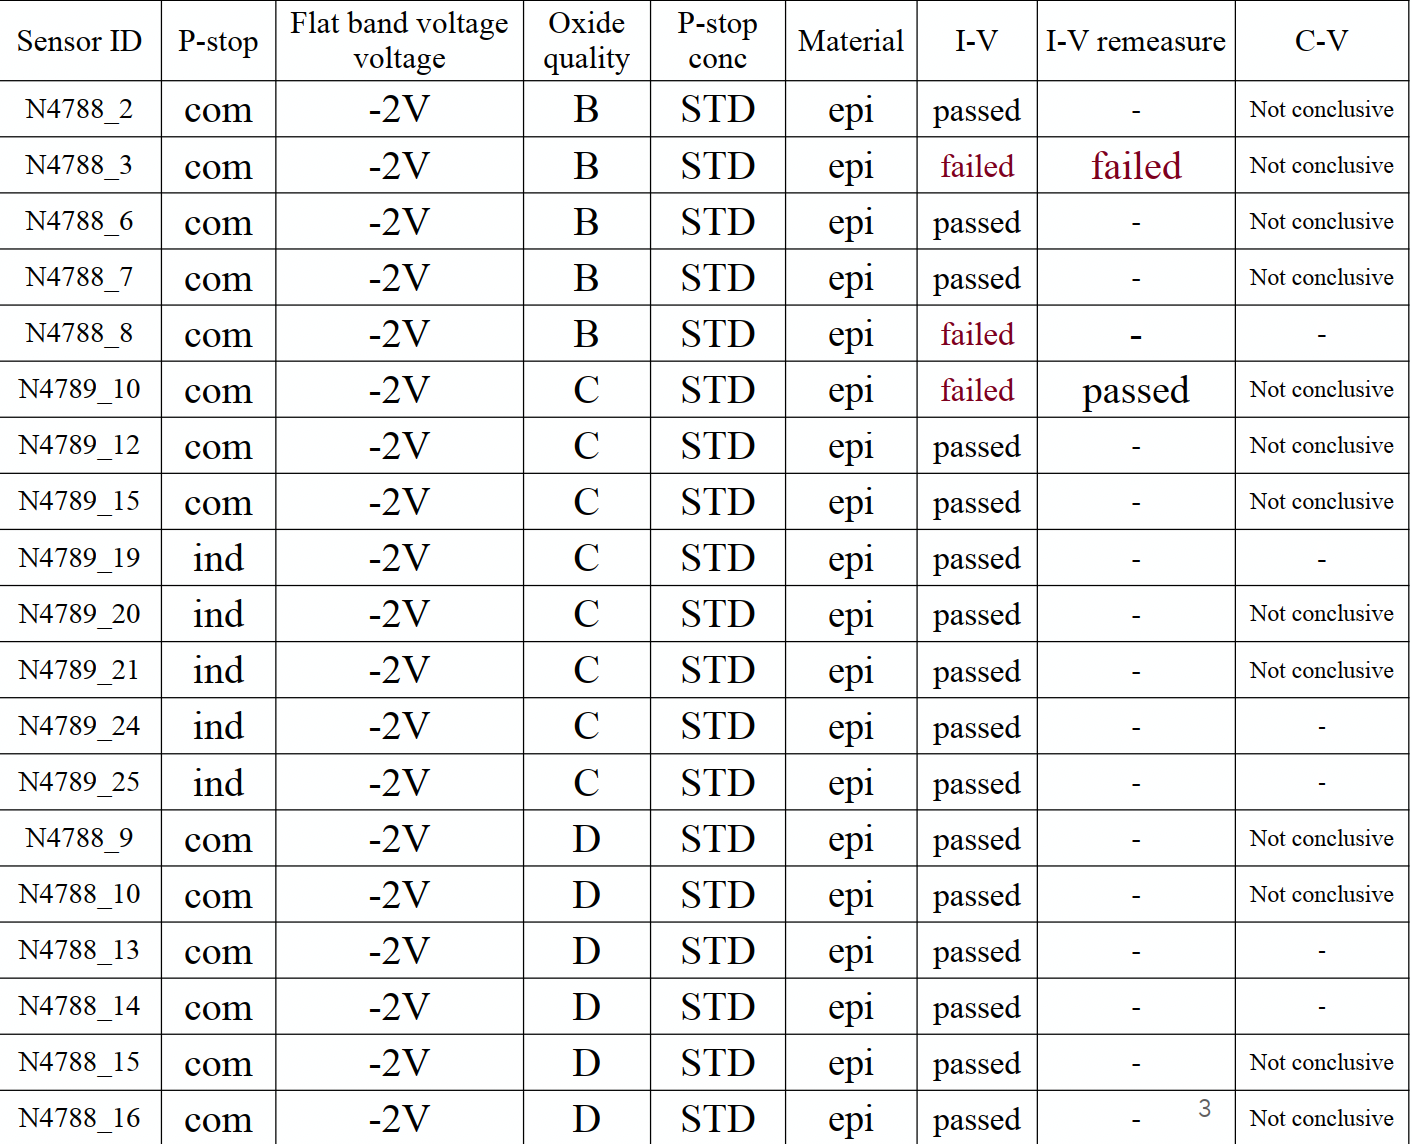
\includegraphics[width=.8\textwidth]{plots/PM8_sensorList.png}
%    \end{figure} 
% \end{frame}


% \begin{frame}{Sensor list: LD}
%    \begin{figure}
%        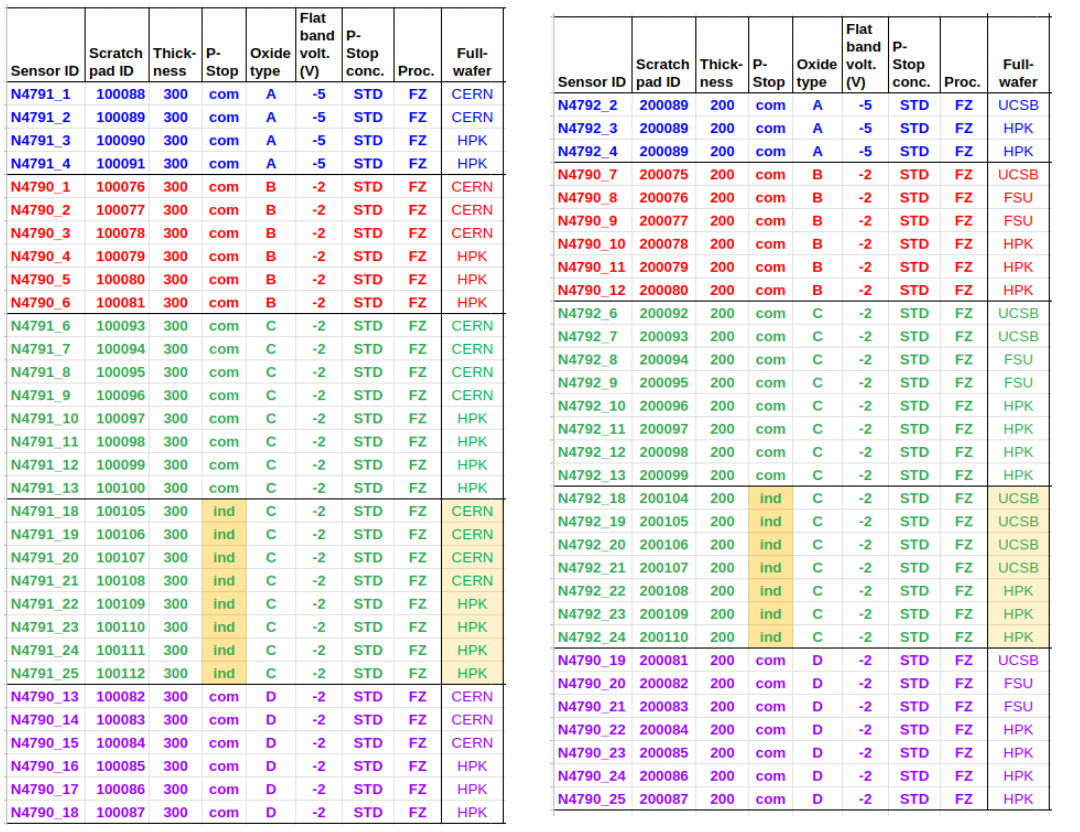
\includegraphics[width=.8\textwidth]{plots/Fall_2021_sensorList.png}
%    \end{figure} 
% \end{frame}

% \begin{frame}{Proto-A, 120 um, CV results: HPK and CERN}
%   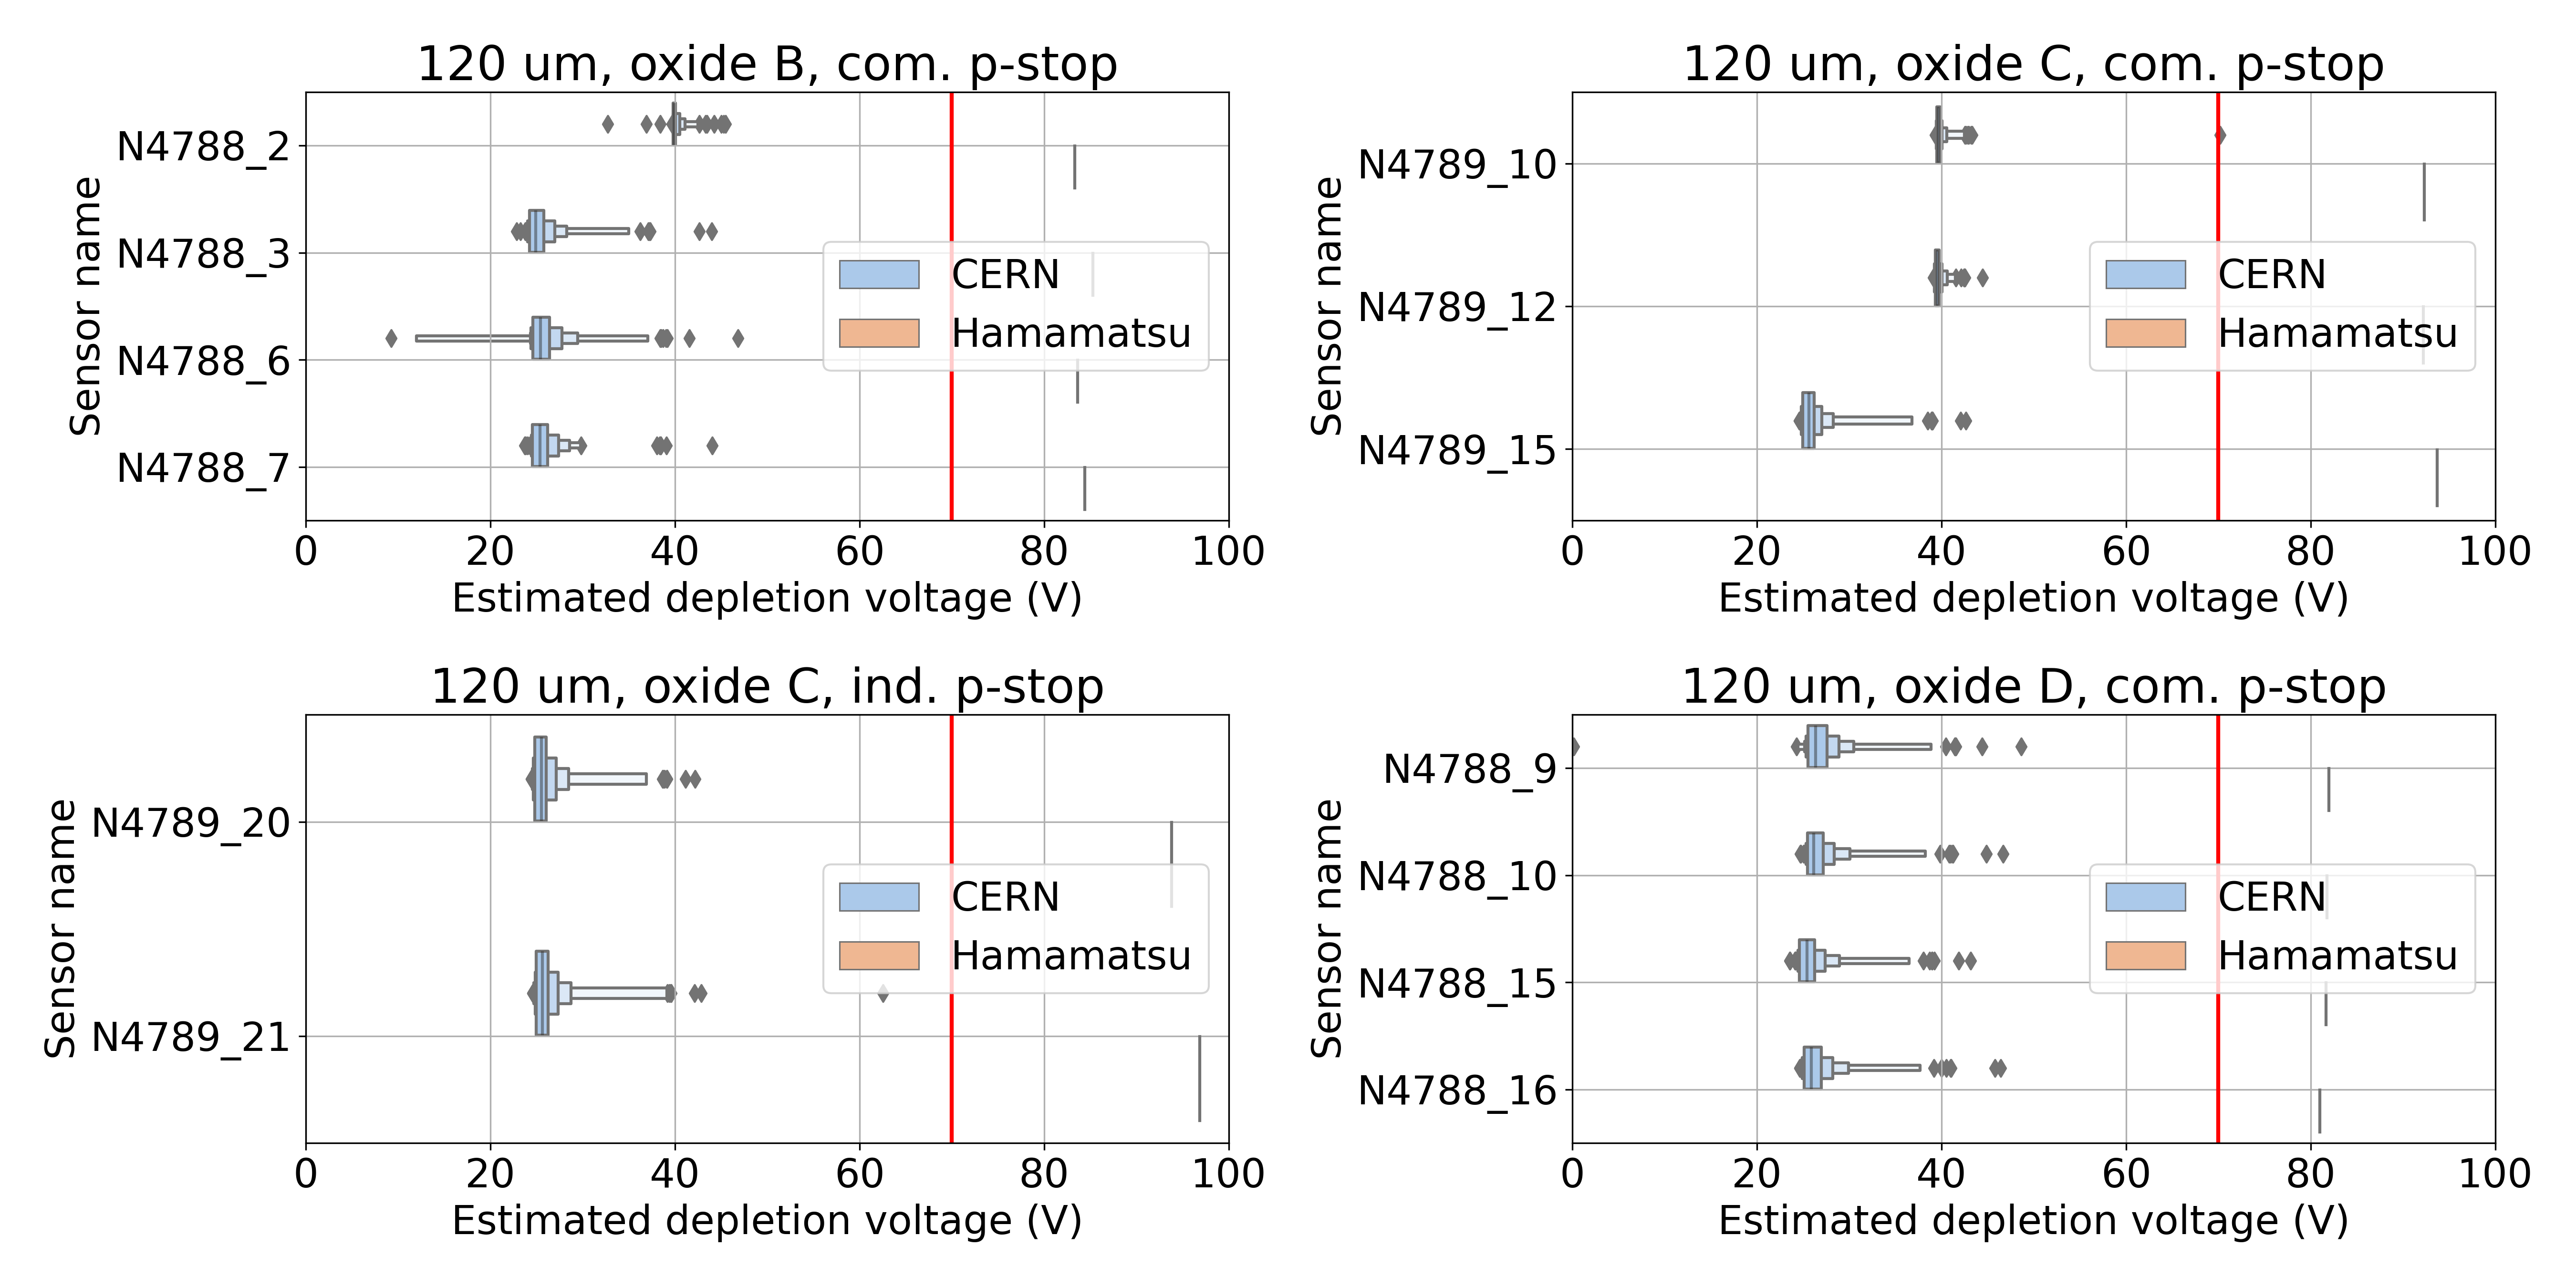
\includegraphics[width=.8\textwidth]{plots/CV_ComparisonHPKCERN_120um.png}
%   \begin{block}{}
%     \begin{itemize}
%       % \scriptsize
%       \item Hamamatsu results are outside the treshhold. CERN results are good.
%       \item Hamamatsu measures one diode, while CERN measures all channels.
%       \item Hamamatsu measures on Dicing Frame, which CERN off Dicing Frame.
%     \end{itemize}
%   \end{block}
% \end{frame}
% \begin{frame}{Proto-A, 200 um, CV results: HPK and CERN (on DF)}
%   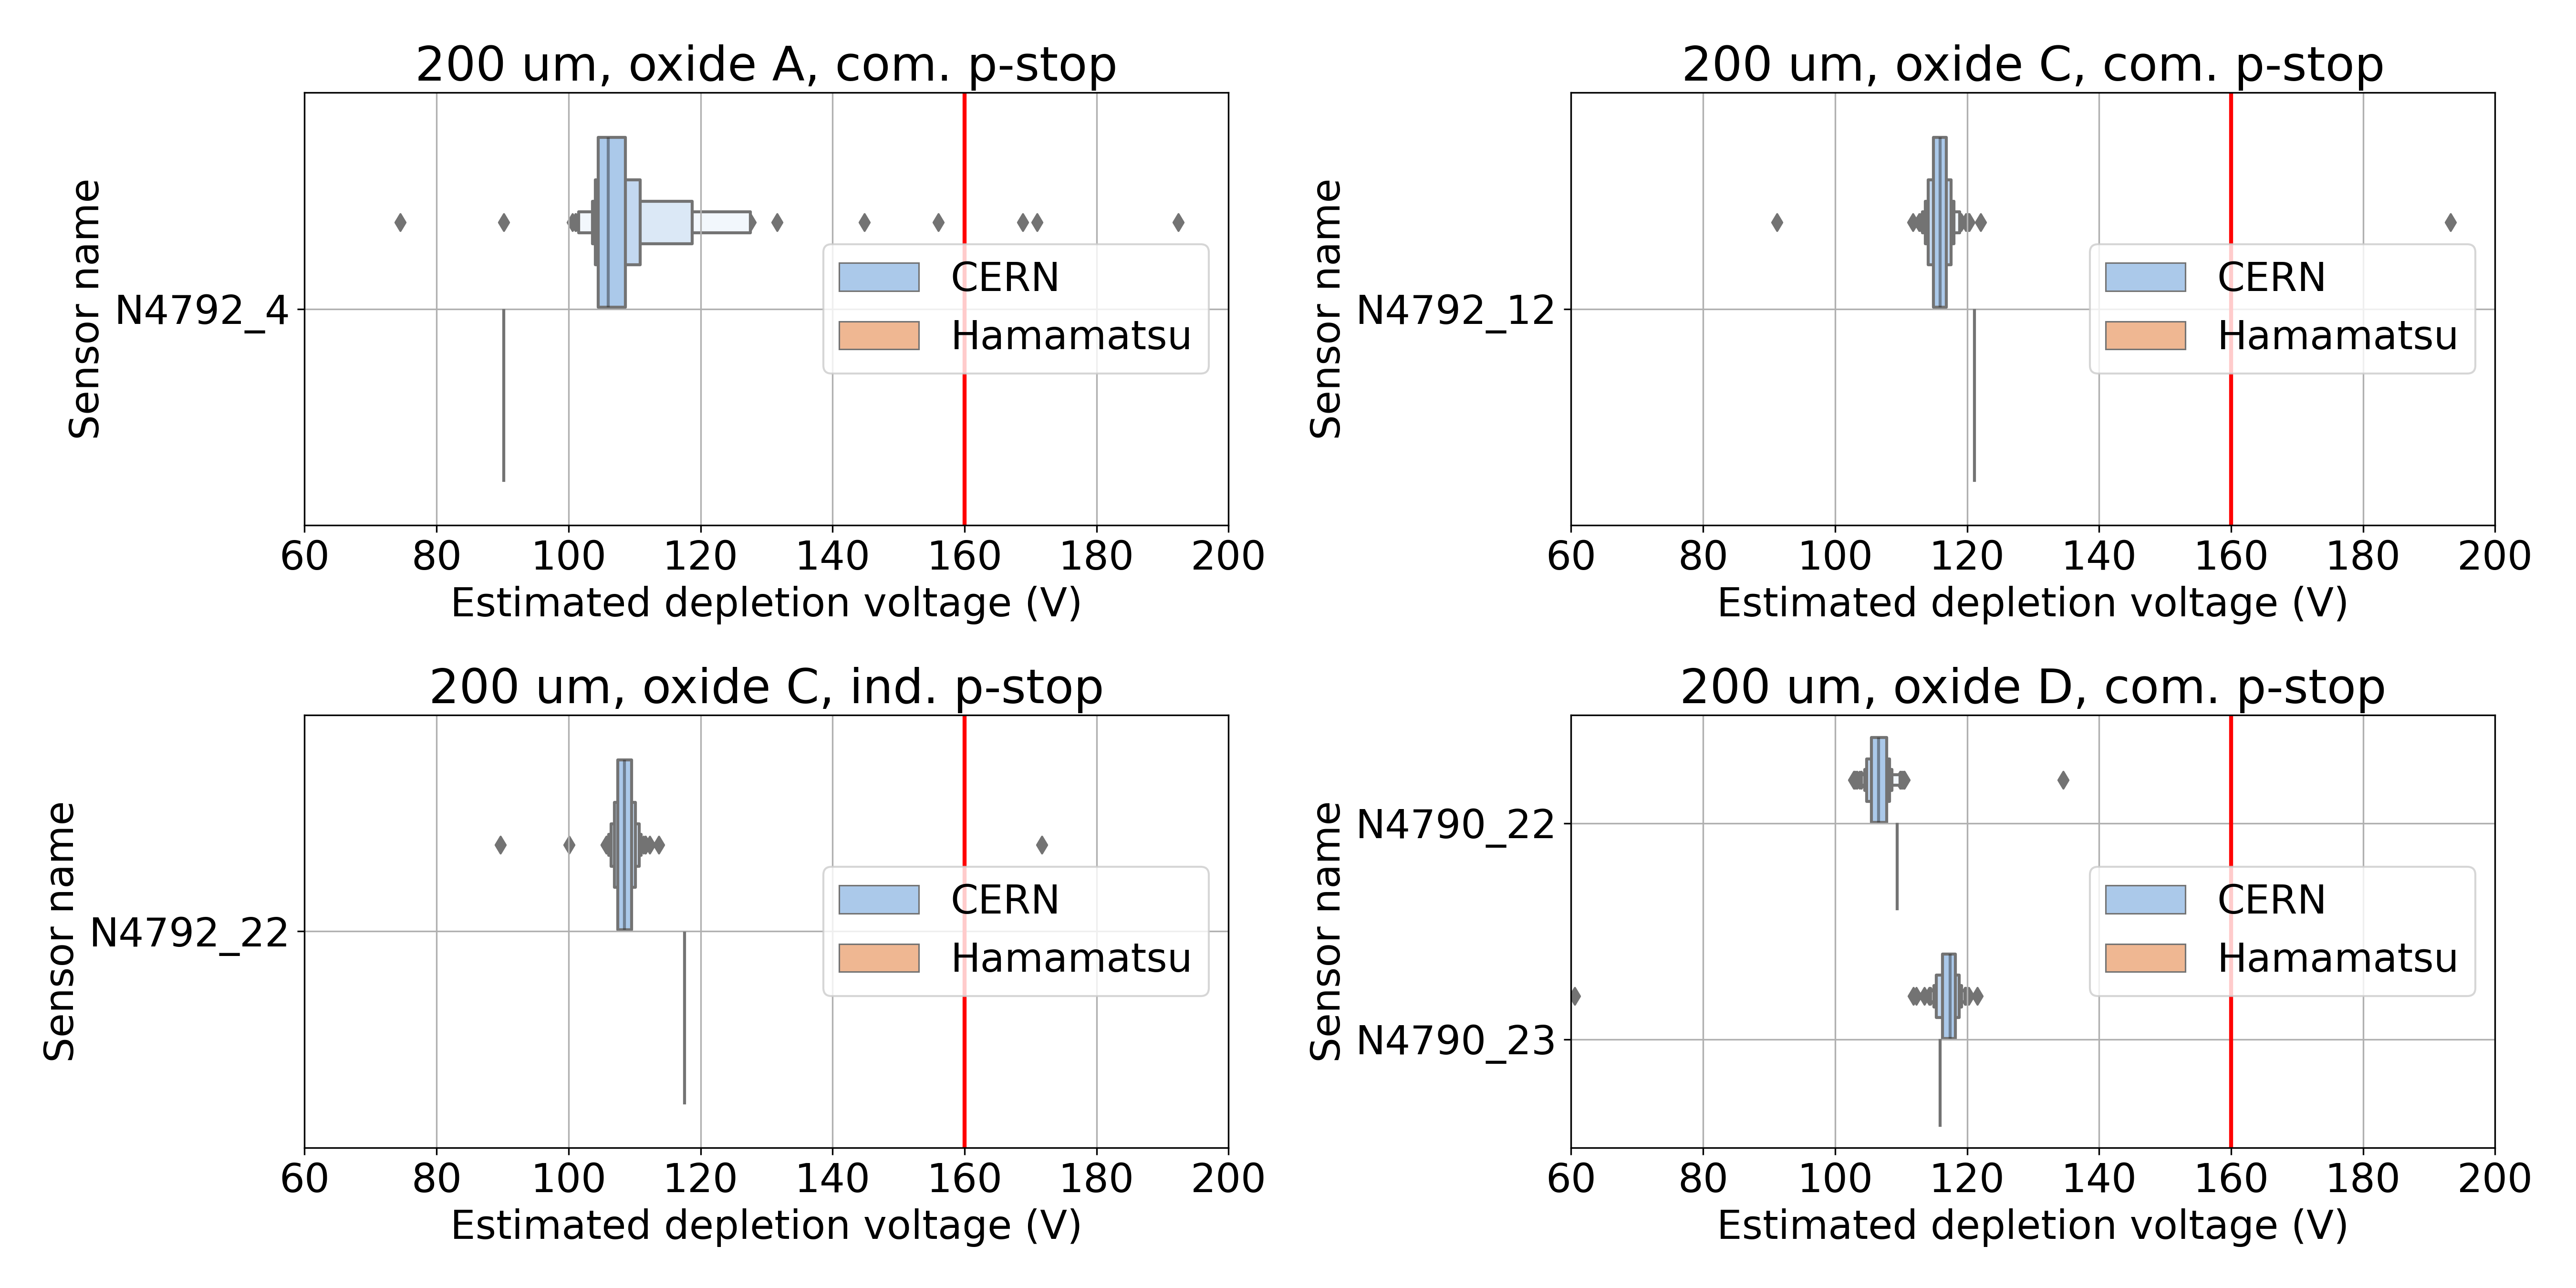
\includegraphics[width=.9\textwidth]{plots/CV_ComparisonHPK_200um.png}
%   \href{https://indico.cern.ch/event/1132823/contributions/4755812/attachments/2399581/4103704/LD\%20proto-A\%20sensors\%20200\%20um\%2C\%20ALPS\%20Winter\%202022.pdf}{\beamergotobutton{Proto-A, 200 um}}
% \end{frame}

% \begin{frame}{Proto-A, 200 um, IV grading (all passed)}
%   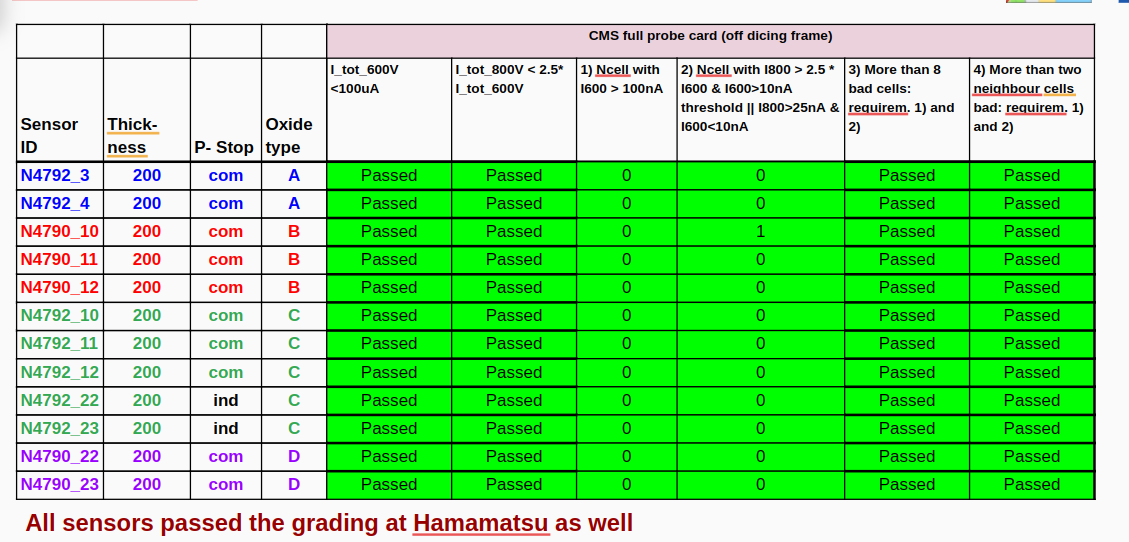
\includegraphics[width=.7\textwidth]{plots/IV_grading_200um.png}
% \end{frame}


% \begin{frame}{Proto-A, 300 um, IV results}
%   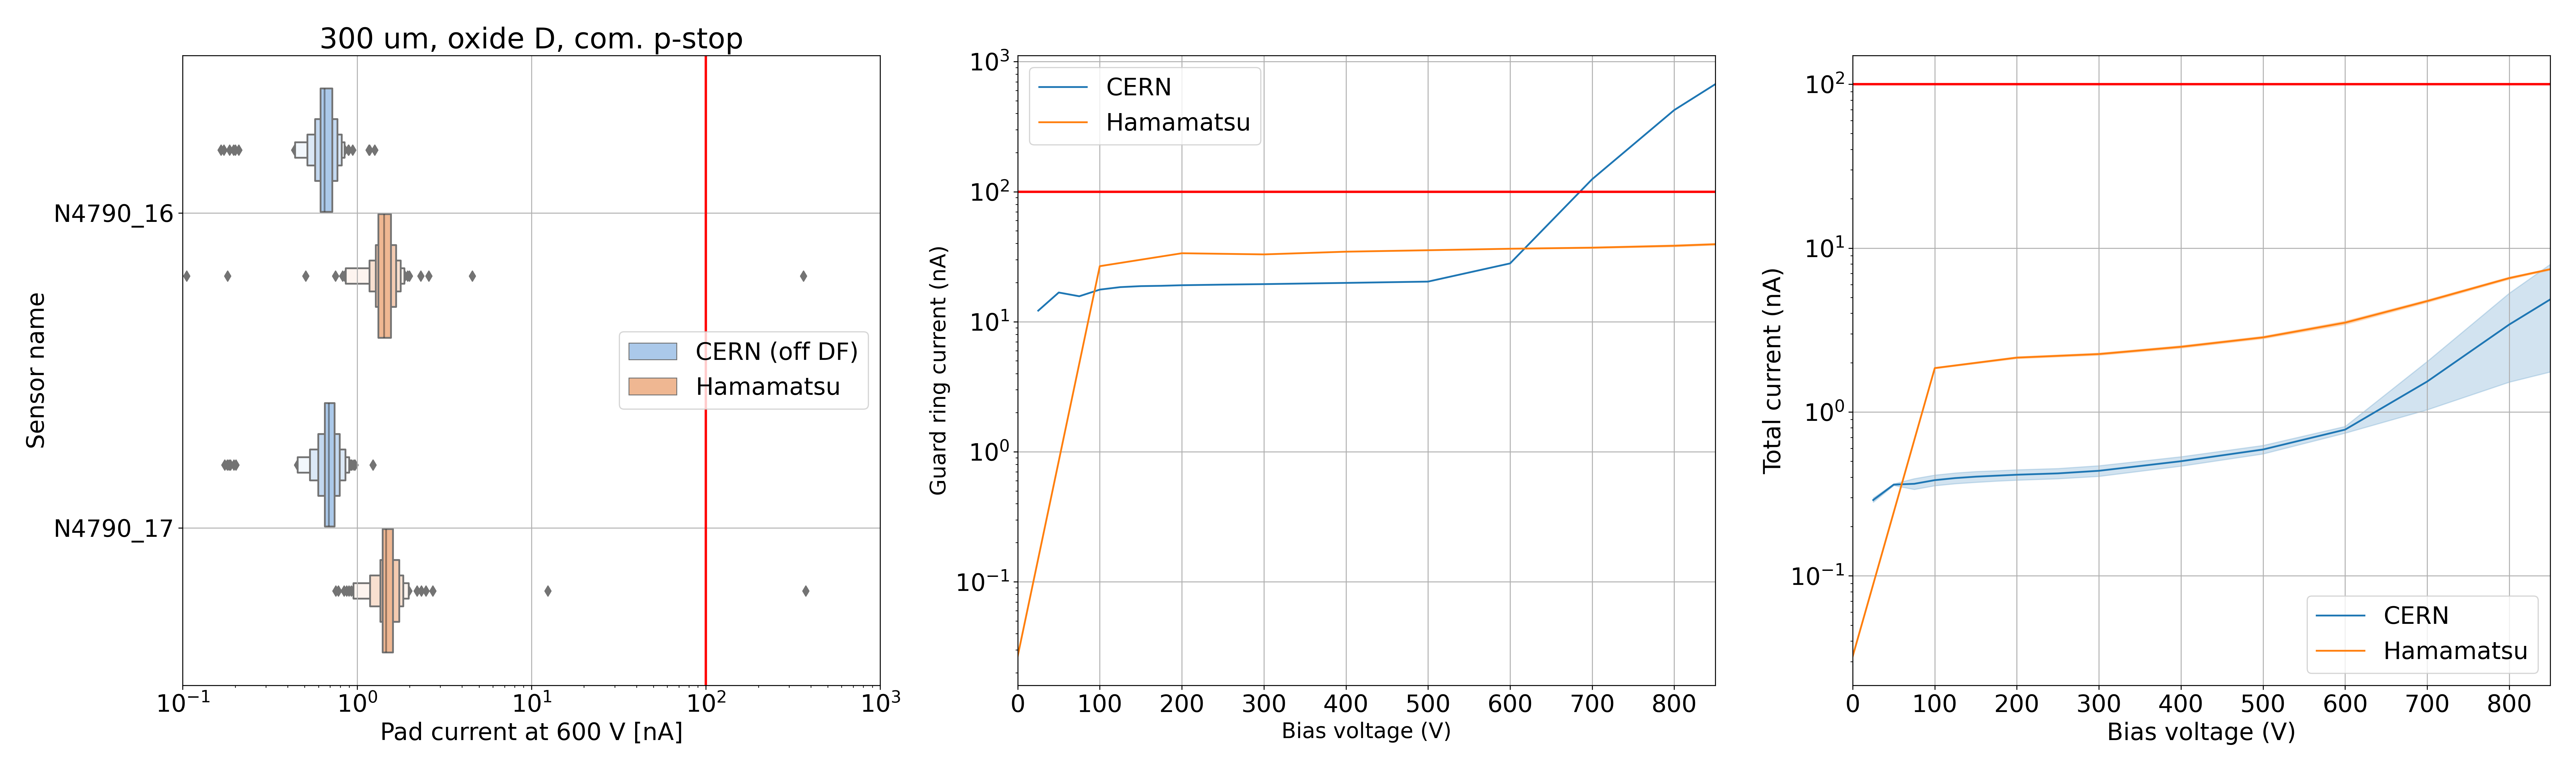
\includegraphics[width=.7\textwidth]{plots/IV_Comparison_SensorsHPK_300um.png}
% \end{frame}

% \begin{frame}{Proto-A, 300 um, IV grading comparison}
%   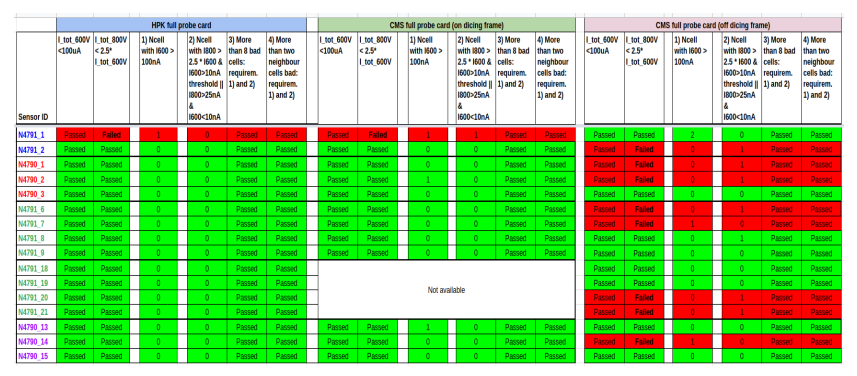
\includegraphics[width=.7\textwidth]{plots/IV_grading_300um.png}
% \end{frame}


% \begin{frame}{Proto-A, 200 um, CV grading (all passed)}
%   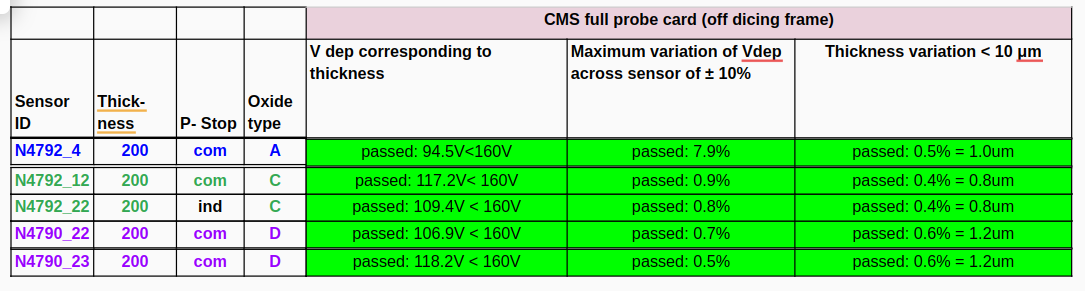
\includegraphics[width=.7\textwidth]{plots/CV_grading_200um.png}
% \end{frame}

% \begin{frame}{Proto-A, 300 um, CV grading comparison}
%   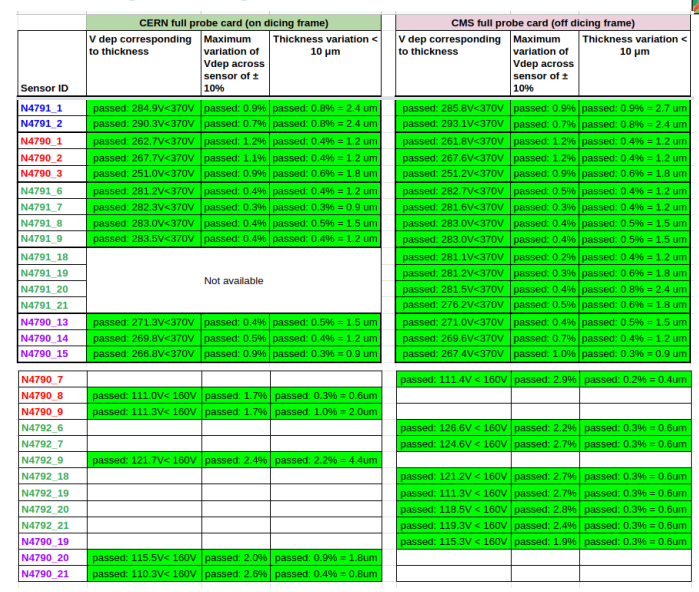
\includegraphics[width=.7\textwidth]{plots/CV_grading_300um.png}
% \end{frame}

% \begin{frame}{Proto-A Batch 2, 300 um, CV results: HPK and CERN (on DF)}
%   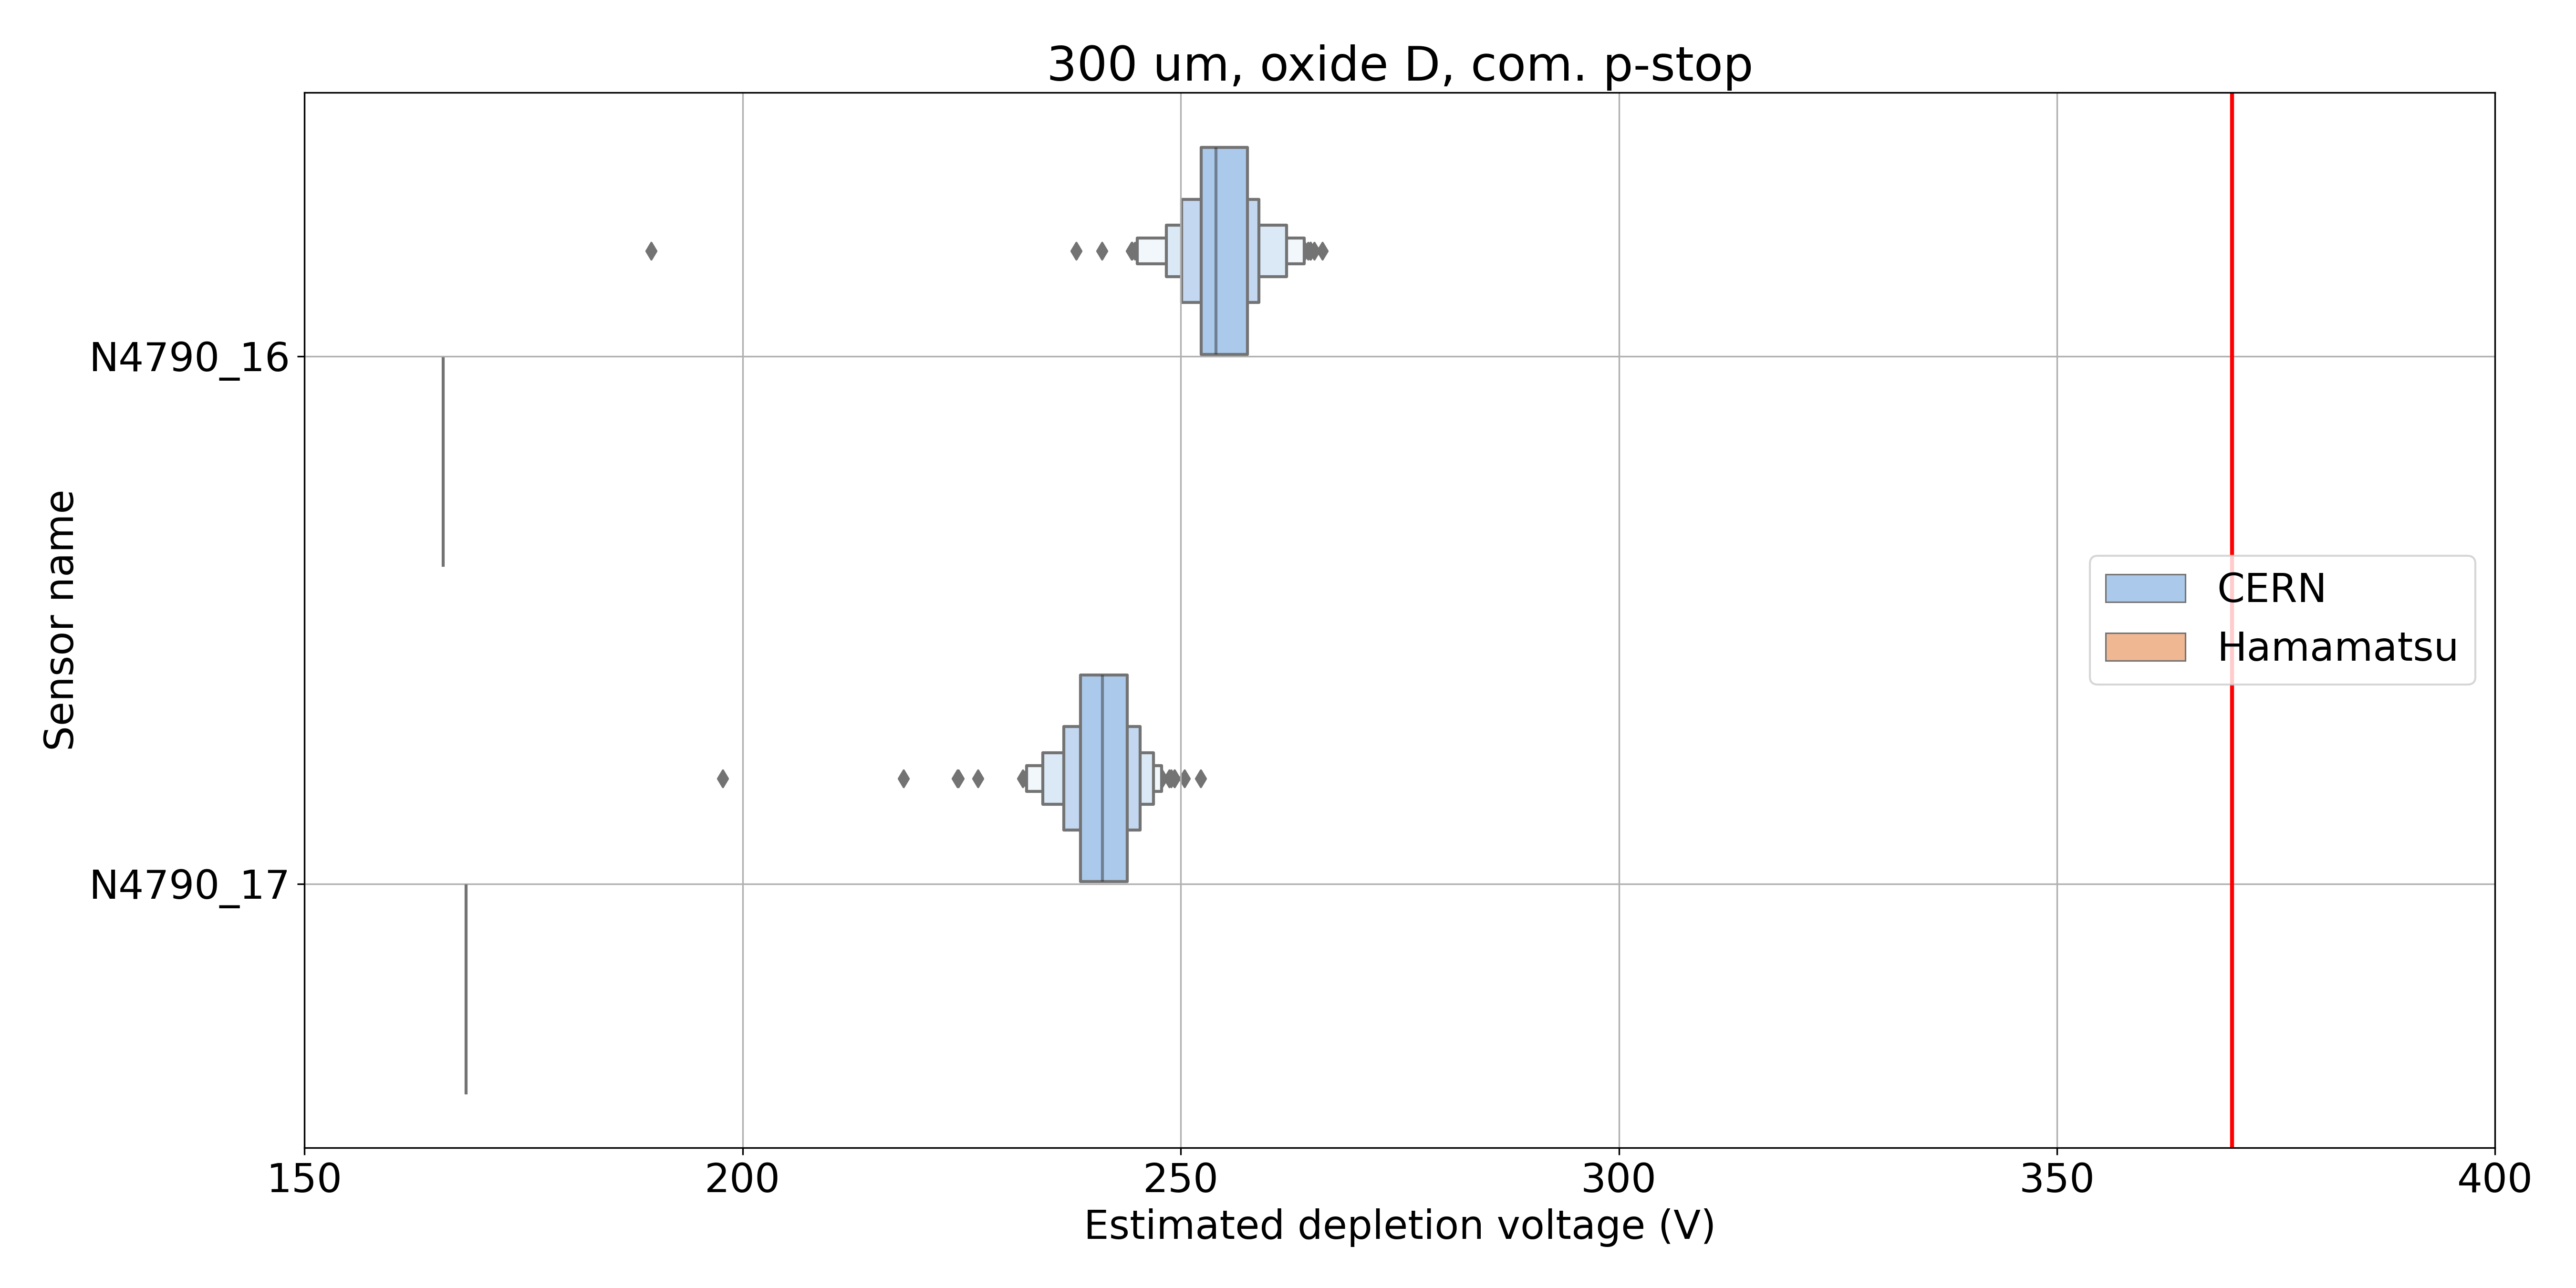
\includegraphics[width=.8\textwidth]{plots/CV_ComparisonHPK_300um.png}
% \end{frame}

% \begin{frame}{Proto-A, Batch 2, 300 um, CV grading comparison}
%   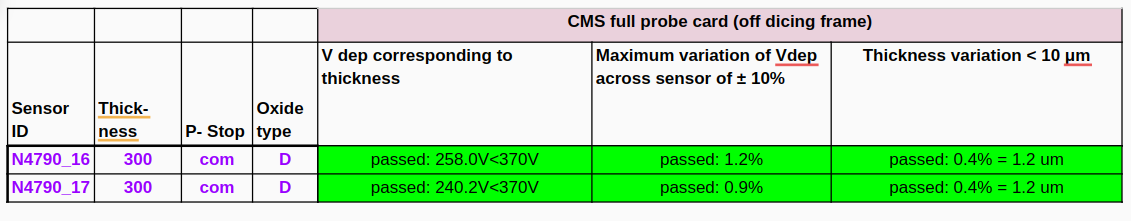
\includegraphics[width=.7\textwidth]{plots/CV_grading_300um_2.png}
% \end{frame}

% \begin{frame}{Proto-A, 120 um, failed fits, cell distribution}
%   \begin{figure}
%     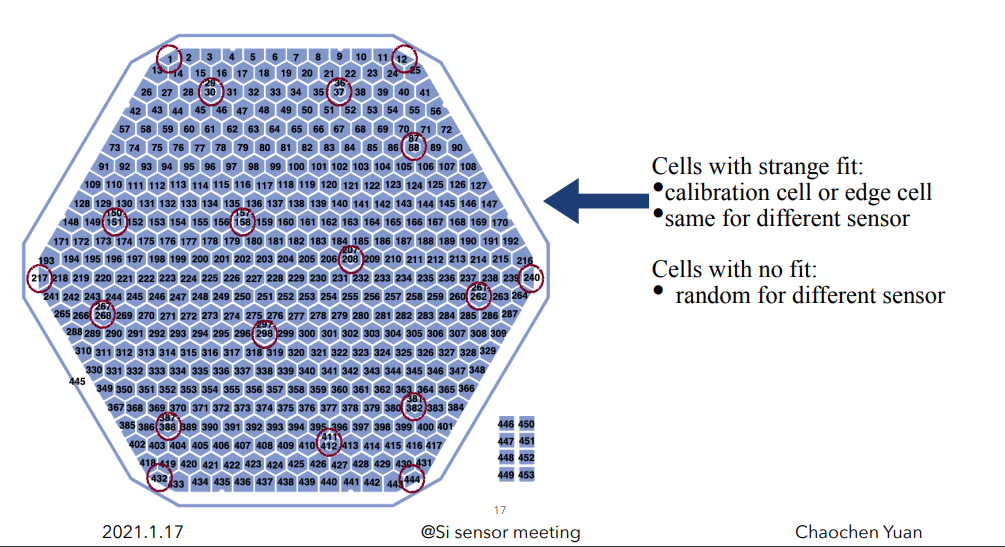
\includegraphics[width=.9\textwidth]{plots/CV_Fit_Distribution.png}
%   \end{figure}
% \end{frame}

% \begin{frame}{Longterm Leakage current stability, sensors}
%   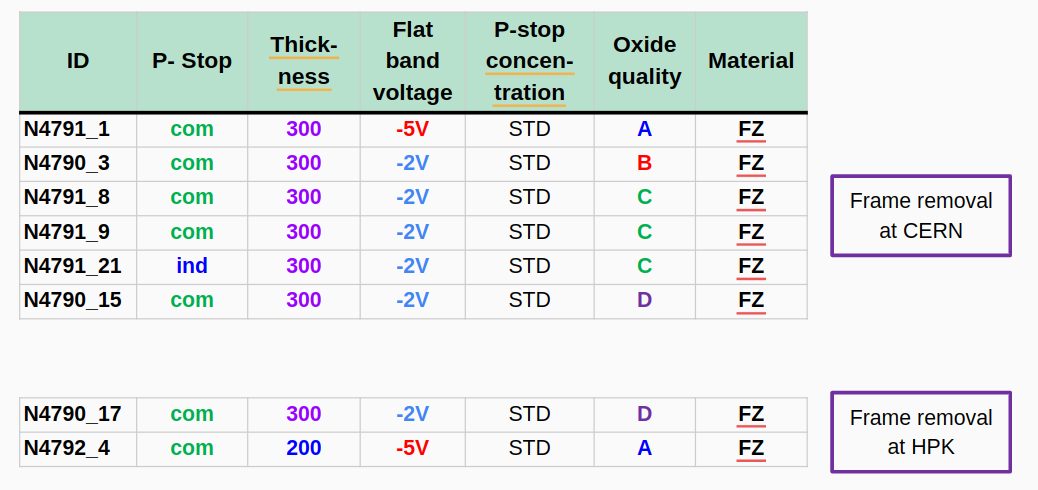
\includegraphics[width=.9\textwidth]{plots/Longterm_sensors.png}
% \end{frame}

% \begin{frame}{Longterm Leakage current stability}
%   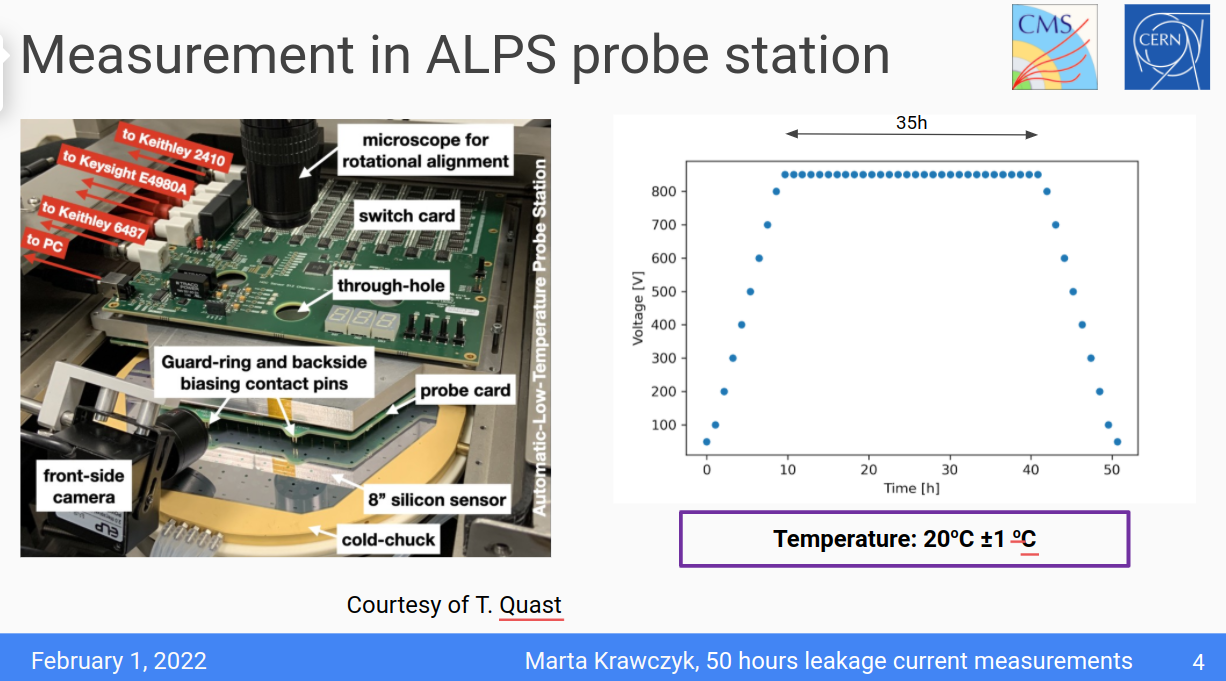
\includegraphics[width=.7\textwidth]{plots/Longterm_process.png}
% \end{frame}

% \begin{frame}{Proto-A: example IV+CV results}
%     \begin{figure}
%   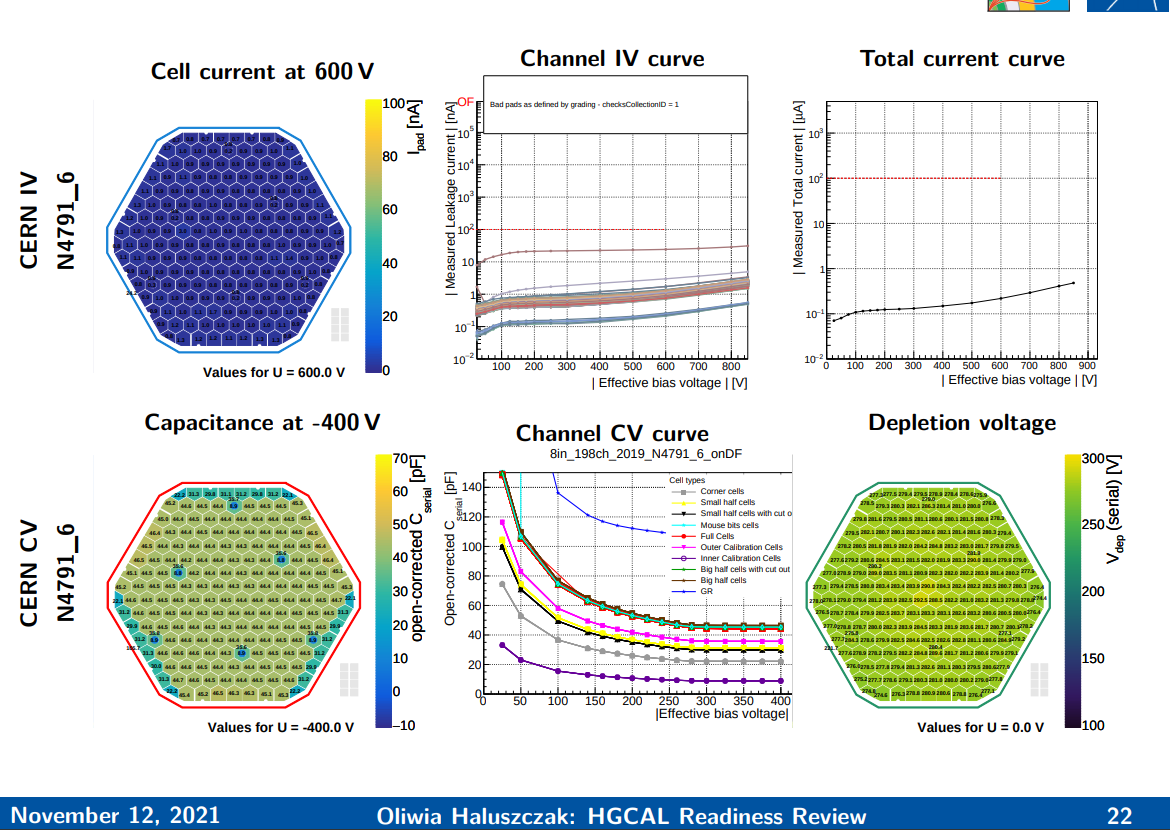
\includegraphics[width=.8\textwidth]{plots/IV_CV_example.png}
        
%     \end{figure}
% \end{frame}

% \begin{frame}{Proto-A: corrected CV fit}
%   \begin{figure}
% 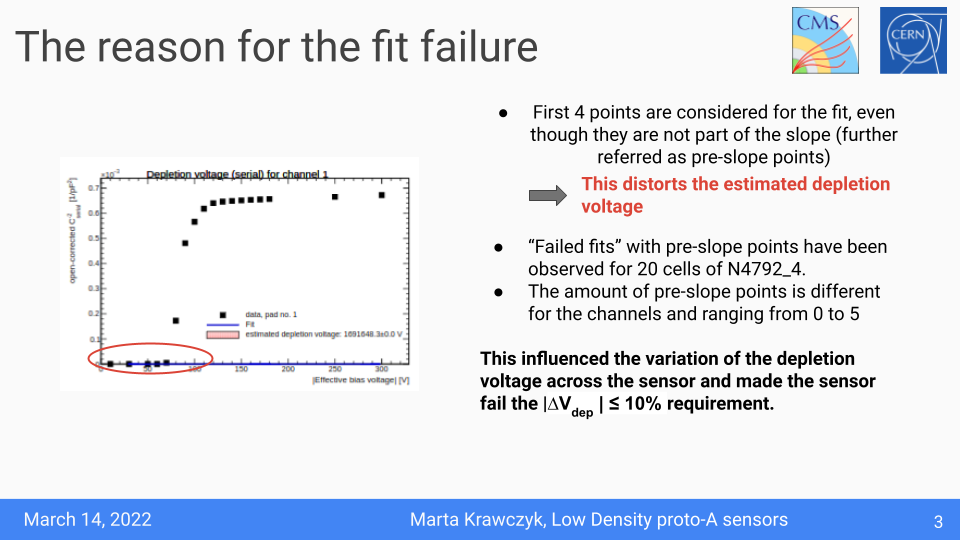
\includegraphics[width=.8\textwidth]{plots/LD_proto-A_sensors_200_um_failed_Vdep_fit.png}     
%   \end{figure}
% \end{frame}

% \begin{frame}{Proto-A: corrected CV fit}
%   \begin{figure}
% \includegraphics[width=.8\textwidth]{plots/LD_proto-A_sensors_200_um_failed_Vdep_fit (1).png}     
%   \end{figure}
% \end{frame}

% \begin{frame}{Proto-A: corrected CV fit}
%   \begin{figure}
% \includegraphics[width=.8\textwidth]{plots/LD_proto-A_sensors_200_um_failed_Vdep_fit (2).png}     
%   \end{figure}
% \end{frame}

% \begin{frame}{Proto-A: corrected CV fit}
%   \begin{figure}
% \includegraphics[width=.8\textwidth]{plots/LD_proto-A_sensors_200_um_failed_Vdep_fit (3).png}     
%   \end{figure}
% \end{frame}


%\begin{frame}
%\frametitle{Sample frame title}
%
%In this slide, some important text will be
%\alert{highlighted} because it's important.
%Please, don't abuse it.
%
%\begin{block}{Remark}
%Sample text
%\end{block}
%
%\begin{alertblock}{Important theorem}
%Sample text in red box
%\end{alertblock}
%
%\begin{examples}
%Sample text in green box. The title of the block is ``Examples".
%\end{examples}
%\end{frame}
%
%\begin{frame}{Make Titles Informative.}
%  You can create overlays\dots
%  \begin{itemize}
%  \item using the \texttt{pause} command:
%    \begin{itemize}
%    \item
%      First item.
%      \pause
%    \item    
%      Second item.
%    \end{itemize}
%  \item
%    using overlay specifications:
%    \begin{itemize}
%    \item<3->
%      First item.
%    \item<4->
%      Second item.
%    \end{itemize}
%  \item
%    using the general \texttt{uncover} command:
%    \begin{itemize}
%      \uncover<5->{\item
%        First item.}
%      \uncover<6->{\item
%        Second item.}
%    \end{itemize}
%  \end{itemize}
%\end{frame}
%
%
%% All of the following is optional and typically not needed. 
%\appendix
%\section<presentation>*{\appendixname}
%\subsection<presentation>*{For Further Reading}
%
%\begin{frame}[allowframebreaks]
%  \frametitle<presentation>{For Further Reading}
%    
%  \begin{thebibliography}{10}
%    
%  \beamertemplatebookbibitems
%  % Start with overview books.
%
%  \bibitem{Author1990}
%    A.~Author.
%    \newblock {\em Handbook of Everything}.
%    \newblock Some Press, 1990.
% 
%    
%  \beamertemplatearticlebibitems
%  % Followed by interesting articles. Keep the list short. 
%
%  \bibitem{Someone2000}
%    S.~Someone.
%    \newblock On this and that.
%    \newblock {\em Journal of This and That}, 2(1):50--100,
%    2000.
%  \end{thebibliography}
%\end{frame}

\end{document}


